\documentclass[11pt, a4paper, twoside]{article}

% --- Packages ---

\usepackage[ngerman]{babel}
\usepackage[a4paper,top=2cm,bottom=2cm,inner=2.75cm,outer=2.75cm,marginparwidth=1.75cm]{geometry}
\usepackage{amsmath}
\usepackage{caption}
\usepackage{setspace}
\usepackage{float}
\usepackage{acronym}
\usepackage{makecell}
\usepackage{tikz}
\usepackage{xcolor}
\usepackage{tcolorbox}
\usepackage{parskip}
\usepackage{pdfpages}
\usepackage{longtable}
\usepackage{array}
\usepackage{booktabs}
\usepackage[backend=biber, style=authoryear]{biblatex}
\usepackage{hyperref}
\usepackage{fancyhdr}
\usepackage{listings}
\usepackage[utf8]{inputenc}
\usepackage[T1]{fontenc}
\usepackage{color}
\usepackage{graphicx}
\usepackage{amsfonts}
\usepackage{nameref}
\usepackage{enumitem}
\usepackage{csquotes}

% --- command rearrangement ---

\let \cite\parencite
\newcommand{\titleref}[1]{(\nameref{#1})}
\newcommand{\titlerefN}[1]{\nameref{#1}}

% --- declaration ---

% Changes citation brackets to square brackets
\DeclareCiteCommand{\parencite}[\mkbibbrackets]
  {\usebibmacro{prenote}}
  {\usebibmacro{citeindex}%
   \printtext[bibhyperref]{\printnames{labelname} \printfield{year}}}
  {\multicitedelim}
  {\usebibmacro{postnote}}

\definecolor{captiongray}{gray}{0.4}
\DeclareCaptionFont{captiongray}{\color{captiongray}\footnotesize}
\captionsetup[figure]{font=captiongray, labelfont=captiongray}
\captionsetup[table]{font=captiongray, labelfont=captiongray}

% --- Fonts ---

\renewcommand{\rmdefault}{ptm}  % Times New Roman
\renewcommand{\sfdefault}{phv}  % Helvetica

% --- Code Listing Style ---

\definecolor{codegreen}{rgb}{0,0.6,0}
\definecolor{codegray}{rgb}{0.5,0.5,0.5}
\definecolor{codepurple}{rgb}{0.58,0,0.82}
\definecolor{backcolour}{rgb}{0.95,0.95,0.92}

\lstdefinestyle{mystyle}{
    backgroundcolor=\color{backcolour},
    commentstyle=\color{codegreen},
    keywordstyle=\color{magenta},
    numberstyle=\tiny\color{codegray},
    stringstyle=\color{codepurple},
    basicstyle=\ttfamily\footnotesize,
    breakatwhitespace=false,
    breaklines=true,
    captionpos=b,
    keepspaces=true,
    numbers=left,
    numbersep=5pt,
    showspaces=false,
    showstringspaces=false,
    showtabs=false,
    tabsize=2,
    language=Python
}

\lstset{
    style=mystyle,
    literate=
        {Ö}{{\"O}}1 {Ä}{{\"A}}1 {Ü}{{\"U}}1 {ß}{{\ss}}1
        {ü}{{\"u}}1 {ä}{{\"a}}1 {ö}{{\"o}}1 {~}{{\textasciitilde}}1
}

\addbibresource{literatur.bib}

% --- Header and Footer ---

\pagestyle{fancy}
\fancyhf{ }
\lhead{Hochschule Düsseldorf}
\cfoot{\thepage}
\rhead{878007}
\fancyhead[LE]{Hochschule Düsseldorf}
\fancyhead[RO]{878007}
\fancyhead[LO]{Hochschule Düsseldorf}
\fancyhead[RE]{878007}
\renewcommand{\headrulewidth}{0.5pt}
\renewcommand{\footrulewidth}{0.5pt}
\raggedbottom

% --- Document Start ---

\begin{document}

% --- Title Page ---

\pagestyle{empty}
\begin{titlepage}
    \thispagestyle{empty}

    % Bilder links und rechts ausrichten, etwas mehr Abstand nach außen und oben
    \vspace*{1cm} % Abstand von der oberen Kante
    \begin{minipage}{0.45\textwidth}
        \raggedright
        
\includegraphics[width=0.7\textwidth]{Graphics/HSDLogo} % Etwas größere Breite
    \end{minipage}%
    \hfill
    \begin{minipage}{0.45\textwidth}
        \raggedleft
        
\includegraphics[width=0.7\textwidth]{Graphics/FacultyOfMedia} % Etwas größere Breite
    \end{minipage}

    \vspace{1.5cm} % Abstand nach den Logos

    \center

    \textsc{\Large wissenschaftliche Vertiefung}\\[2cm]

    \huge{Der Fortschritt}\\[0.2cm]
    \huge{automatischer Musiktranskriptionssysteme}\\[0.2cm]
    \huge{durch künstliche Intelligenz}\\[2cm]
    \Large

    % Informationen untereinander zentrieren
    \begin{center}
        \textit{Autor:} \\
        Benedikt Kolodziej \\
        878007 \\
        Medieninformatik (B. Sc.) \\[1cm]

        \textit{Betreuender Professor:} \\
        Prof. Dr. Dennis Müller\\
        dennis.mueller@hs-duesseldorf.de \\[1cm]

        \textit{Zeitraum} \\
        28.05.2025 - xy
    \end{center}

    \vspace{3cm} % Weniger Abstand vor dem Unterschriftenbereich

    %\begin{flushleft}
    %    Unterschrift Praxisstellenbetreuung
    %    \vspace{0.5in}

    %    \rule{0.3\textwidth}{0.4pt} \hspace{1cm} \rule{0.3\textwidth}{0.4pt}\\
    %    \makebox[0.3\textwidth][l]{Ort, Datum} \hspace{1cm} \makebox[0.3\textwidth][l]{Unterschrift}
    %\end{flushleft}
\end{titlepage}



\newpage

% --- Table of Contents and Lists ---

\setcounter{tocdepth}{3}
\tableofcontents
\newpage

\listoffigures
\listoftables
\newpage

% --- Main Content ---

\pagestyle{fancy}
\setcounter{page}{1}
\pagenumbering{arabic}

\section{Einleitung}
Hier kommt deine Einleitung hin. Du kannst diese Datei einfach weiter schreiben.
 % Korrigiert
\section{Geschichtliche Entwickelung von AMT-Systemen}

\subsection{Moorer und eines der ersten Musiktranskriptionssysteme}
\subsubsection{Grundlegende Probleme bei AMTs}
Einer der ersten Papers über Automatic Music Transcription wurde von James A. Moorer im Jahr 1977 geschrieben.
\cite{Moorer1977}
In diesem beschreibt Moorer seinen Ansatz, polyphone Musik Audiospuren
direkt über Computerprogramme in Notenschrift zu übertragen.
Während dieses Prozesses fallen ihm schon sehr viele schwierigkeiten auf, die auch in späteren Papern und Arbeiten
eine ausschlaggebende Rolle spielen werden.

Eines dieser Probleme wird von ihm als das \("\)Cocktail-Party-Problem\("\) bezeichnet.
Dieses stellt die Schwierigkeit dar, auf einer Party bestimmten Stimmen zu folgen, während viele verschiedene Stimmen
gleichzeitig erklingen.
Das gleiche Problem liegt in der Noten transkription.
Die meisten Musikstücke haben mehrere Instrumente, welche gleichzeitig spielen.
Öfter gibt es auch Musikstücke wo es für ein Instrument, wie zum Beispiel Violine, mehrere verschiedene Stimmen gibt.
Dies erschwert die Zuordnung bestimmter Noten zu einer gewählten Stimme.
Schon viele Menschen scheitern deshalb daran große Musikstücke richtig zu transkribieren.
Noch schwieriger wird es hier für Computerprogramme.
Anfangs identifizieren diese bestimmte Töne anhand der Frequenz des Tons.
Leider reicht das, wie Moorer feststellt, nicht aus um genaustens zu bestimmen,
welche Töne genau momentan gespielt werden.

Jeder Ton hat Obertöne.
Diese Obertöne sind jeweils das Vielfache von dem Grundton, den man spielt.
Heißt, wenn ich auf einem Klavier den Ton C3 mit 130,81 Hz spiele dann hat dieser
die Obertöne C4 (261,62 Hz), G4 (392,42 Hz) usw.
Wenn man nur C3 spielt erklingen für das Computerprogramm auch die jeweiligen Obertöne,
was man Frequenzüberlagerung nennt.
Diese Frequenzüberlagerung sorgt dafür, das zum Beispiel ein Klavier anders klingt als eine Violine.
Daraus resultiert dann die Klangfarbe (Timbre) eines bestimmten Instrumentes.
\cite{goswami2013timbre}
Leider konnte Moorer zu dieser Zeit noch nicht die Klangfarbe eines Instruments erkennen.
Er konnte auch noch nicht das Problem der Obertöne lösen,
da die damaligen Algorithmen und Verfahren noch nicht in der Lage waren die Grundfrequenz von den Obertönen zu trennen,
weshalb er sich ausschließlich auf zweistimmige polyphone Musikstücke fokussierte.

Ein weiteres Problem war Rauschen in realistischen Audiospuren und
Stilistische mittel in der Musik, wie zum Beispiel Vibrato.
In real aufgenommenen Audiospuren gibt es immer ein gewisses Hintergrundrauschen.
\cite{iZotope2025noisefloor}
Dieses kann von einem Computerprogramm auch als Note erkannt werden oder verhindern, das bestimmte Noten
richtig vom Computerprogramm erkannt werden.
Moorer hat ein Musikstück analog aufgenommen und dieses dann mit einem 14-Bit converter digitalisiert.
Dadurch war das Rauschen nicht weg, aber da er das Musikstück selber aufgenommen hat und dieses konvertiert hat
sorgte es für insgesamt geringeres Rauschen.
Zudem konnte er so die Musiker davon abhalten bestimmte Stilistische mittel zu verwenden,
um bessere Daten zur Transkription zu erhalten.
Stilistische mittel, wie Vibrato, konnten nicht genutzt werden,
da diese eine kleine aber kontinuierliche Veränderung der Frequenz verursachen.
Dadurch kann das Computerprogramm nicht korrekt erkennen, das eigentlich eine einzelne Note gespielt wurde.
Somit war der Onset und Offset der Note komplett falsch.

Das letzte Problem, was Moorer angesprochen hat, ist das Nutzen von nicht
harmonischen Instrumenten wie Trommeln oder einem Schlagzeug.
Diese Instrumente haben keinen eindeutigen Pitch für deren Töne,
sie sind eher abhängig von Rhythms und Lautstärke.
Da Moorers AMT sich jedoch auf das Frequenzmuster der Noten fokussiert,
können diese Musikinstrumente nicht berücksichtigt werden.

\subsubsection{Der Aufbau von Moorers AMT-Systems}
Moorers automatische Musiktranskriptionssystem war eins der ersten seiner Art.
Viele weiteren AMT-System leiten sich von diesen ab.

Zunächst wird ein analoges Musiksignal mit einem 14-Bit converter digitalisiert.
Dieses digitale Musiksignal wurden dann genutzt um mithilfe von Bandpassfiltern,
ein Filter welcher nur bestimmte Frequenzen durchlässt,
bestimmte Frequenzbereiche zu isolieren.
Dadurch konnte Moorer die gespielte Note und deren Dauer,
also zugleich auch deren Onset und Offset, feststellen.

Nun mussten die bestimmten Noten einer gewählten Stimme zugeordnet werden.
Dies wurde durch melodische Gruppierung verwirklicht.
Zunächst wurden Inseln gebildet.
Inseln sind Noten die sich Zeitlich vollständig überlappen.
Wir gehen davon aus das jede Stimme nur eine Note gleichzeitig spielt,
wodurch diese Noten nicht der gleichen Stimme zugeordnet werden können.
Als Nächstes müssen die anderen Noten auf verschiedene Kombinationen getestet werden.
Desto kleiner die Frequenz sprünge je Note sind, desto wahrscheinlicher gehören sie einer Stimme zu.
Zudem werden Gruppierungen von Noten erstellt, welche am wahrscheinlichsten harmonisch nacheinander gespielt worden.

Zum Schluss ließ Moorer die gewonnenen Daten durch ein Programm laufen, 
um diese dann mithilfe eines Plotters in eine Notenschrift umzuwandeln.

\subsubsection{Hidden Markov Models}
Hidden Markov Modelle (HMM) sind statische Modelle, welche sich sehr gut zur Analyse von Musikstücken eignen.
Sie wurden erstmal in den 1960er Jahren erfunden
\cite{baum1970maximization}
und sind ein zentraler bestandteil früherer AMT-Systeme.
HMMs beschreiben eine Abfolge von \("\)versteckten Zuständen\("\),
welche im Kontext von AMT-Systemen Noten im Audiosignal darstellen.
Durch indirekt beobachtbare Daten, wie zum Beispiel die Spektraldaten des Audiosignals,
können diese Noten erschlossen werden.

HMMs bestehen aus:
\begin{itemize}
    \item Zustände (States)
    \item Übergangswahrscheinlichkeiten (Transition Probabilities)
    \item Emissionswahrscheinlichkeiten (Emission Probabilities)
    \item Beobachtungen (Observations)
\end{itemize}
Nehmen wir das Beispiel eines Klaviers.
Ein Klavier hat 88 Tasten, und somit mindestens 88 Zustände.
Durch Akkorde können zudem mehr Zustände generiert werden.
Die Übergangswahrscheinlichkeit stellt dar,
wie wahrscheinliche es ist von einem Zustand zu einem bestimmten anderen Zustand zu wechseln.
Zum Beispiel könnte es wahrscheinlicher sein, dass auf die Note C4 der Ton G3 folgt statt D1,
da diese Tonfolge harmonischer und musikalisch plausibler klingt.
Dies ist jedoch nur eine Annahme anhand von gesammelten Testdaten, weshalb es nicht als Begründung ausreicht.
Deshalb kommt als zweite Instanz die Emissionswahrscheinlichkeit hinzu.
Diese gibt an, wie Wahrscheinlich ein bestimmter Zustand in der momentanen Beobachtung ist.
Die Beobachtung wird dabei zusammengesetzt aus Eigenschaften, wie Frequenzverteilung, Spektrogramm
oder anderen Merkmalen die man aus anderen Modulen herleiten kann.
Aus den gesammelten Daten kann nun mithilfe von zum Beispiel dem Viterbi-Algorithmus
% Quelle
die wahrscheinlichste Abfolge von Zuständen berechnet werden.

\subsection{MIDI-Dateien}
Notenschrift als Input für ein Computerprogramm, Synthesizer oder ähnliches ist unhandlich.
Zunächst müsste man die gespielten Noten immer wieder zu Notenschrift konvertieren
und danach diese auch noch in anderen Programmen analysieren, was sehr aufwändig werden würde.
Eine bessere lösung dafür wäre eine Datenschreibweise,
bei der alle wichtigen Informationen bestimmter Noten übersichtlich aufgeschrieben sind.
MIDI-Dateien sind dafür perfekt geeignet.

MIDI ist ein Standartprotokoll zur kommunikation zwischen
elektronischen Musikinstrumenten, Computern und anderen Geräten wie zum Beispiel Synthesizer.
Dieses Protokoll wurde 1983 erstmals eingeführt und wurde schnell zu einem Standard in der digitalen Musikindustrie.
\cite{smith1983midi}
In MIDI-Dateien werden Daten von Tönen gelagert,
welche zum Beispiel zuvor von einem elektronischen Instrument gespielt wurden oder durch AMTs erfasst wurden.

In MIDI-Dateien werden folgenden Daten gespeichert:
\begin{enumerate}
    \item \textbf{MIDI Header-Chunk (MThd):} Enthält grundlegende Informationen zur Struktur der Datei:
    \begin{itemize}
        \item Formattyp (0 = eine Spur, 1 = mehrere synchrone Spuren, 2 = unabhängige Spuren)
        \item Anzahl der folgenden MTrk-Blöcke (Tracks)
        \item Zeitauflösung (Ticks pro Viertelnote)
    \end{itemize}

    \item \textbf{MIDI Track-Chunks (MTrk):} Jede Spur enthält eine zeitlich sortierte Liste von MIDI-Events:
    \begin{itemize}
        \item \textbf{MIDI-Events:}
        \begin{itemize}
            \item Note Onset / Offset
            \item Control Change (Lautstärke)
            \item Program Change (gibt das spielende Instrument an)
            \item Pitch Bend (verändert die Tonhöhe)
            \item Aftertouch / Polyphonic Key Pressure (Druckstärke pro Taste)
        \end{itemize}
        \item \textbf{Meta-Events:}
        \begin{itemize}
            \item Set Tempo (Tempo in Mikrosekunden pro Viertelnote)
            \item Time Signature (Taktart zum Beispiel 4/4 oder 3/4)
            \item Key Signature (Tonart zum Beispiel C-Dur oder A-Moll)
            \item Track Name
            \item Lyrics
            \item Markers
            \item End of Track (Ende einer Spur)
        \end{itemize}
        \item \textbf{System Exclusive Events (SysEx):}
        \begin{itemize}
            \item Herstellerspezifische Daten wie Synthesizer-Presets oder Spezialbefehle
        \end{itemize}
    \end{itemize}

    \item \textbf{Delta-Time:} Gibt die Zeit (in Ticks) an, die seit dem letzten Event vergangen ist:
    \begin{itemize}
        \item Ermöglicht die genaue zeitliche Positionierung jedes MIDI-Events
        \item Grundlage für das Timing und die rhythmische Struktur der Datei
    \end{itemize}
\end{enumerate}
Am wichtigsten sind dabei die MTrk-Blöcke, in denen die Daten der einzelnen Noten gespeichert werden.
Dabei stellt ein Track die Eventliste einer ganzen Stimme dar,
wie zum Beispiel die Melodiestimme, eine Violine, die Pedalsteuerung eines Klaviers oder Metadaten.
Es fällt auf das diese vier Beispiele alle sehr unterschiedliche Aufgaben und bedeutungen haben.
Das liegt daran, dass in MIDI-Dateien eher zusammenhängende Funktionen gespeichert werden und nicht nur Musiknoten.

MIDI-Dateien kamen auch der Forschung für AMT-Systemen sehr gelegen,
da man nun ein standardisiertes output Format für diese Programme besaß.
Später werden diese zudem sehr Essenziell bei dem Training KI basierter AMT-Systeme.
\cite{telila2025cnn}

\subsection{Polyphone AMT-Systeme und neue Ansätze}
\subsubsection{Blackboard-System}
Moorer stellte, mit seinem AMT-System, viele grundlegende Bausteine für dieses Forschungsgebiet.
Jedoch gab es noch viele offene Probleme, die noch überwunden werden mussten.
Eines der ausschlaggebendsten Probleme stellte sich Keith D. Martin.
\cite{Martin1996}
Zuvor wurden höchstens zwei verschiedene Stimmen gleichzeitig zur Musik transkription verwendet.
Ein großer Teil von Musikstücken verwendet jedoch mehr Stimmen.
Um diese polyphonen Musikstücke zu transkribieren,
baute Martin einen neuen Ansatz eines AMT-Systems mit innovativen Modulen und Ansätzen.

Nachdem das Input Audiosignal in ein Correlogram verarbeitet wurde,
spaltet sich Martins AMT-System auf, in einen Analysepfad und einen Rhythmuspfad.
Dabei konzentriert sich der Analysepfad auf die Zusammenhänge der verschiedenen Noten,
während der Rhythmuspfad sich mehr mit der Lautstärke und den Notenanschlägen beschäftigt.
Am Ende werden diese Kenntnisse zusammengeführt.
Der Output besteht aus dem Onset, der Dauer und der Frequenz jeder gespielten Note.
Martin gibt nicht explizit zurück, welcher Stimme jede Note zugeordnet ist.
Durch das Blackboard-System, und vor allem nach sequentieller Analyse der Intervalle, kann man
jedoch die erhaltenen Noten später bestimmten Stimmen nachträglich korrekt zuordnen.

\begin{figure}[H]
    \centering
    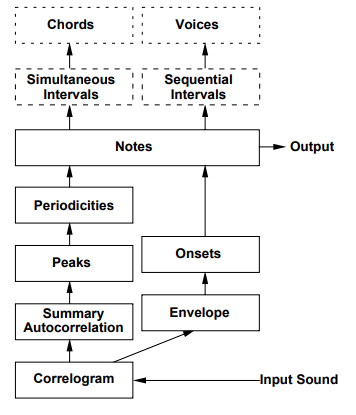
\includegraphics[width=0.6\textwidth]{Graphics/Martin1996Structure}
    \caption{Systemstruktur des AMT-Ansatzes von Keith D. Martin (1996), basierend auf \cite{Martin1996}.}
    \label{fig:martin-structure}
\end{figure}

Martin nutzte ein Blackboard-System zur Notenerkennung und Hypothesenbildung.
Unter anderem kann man dadurch Noten bestimmten Stimmen zuordnen.
Ein Blackboard-System ist ein kollaboratives Problemlösungsmodell, welches aus verschiedenen Modulen besteht,
die alle auf einem gemeinsamen Datenraum Hypothesen aufstellen können.
Um diese Vermutungen aufstellen zu können müssen jedoch erst die dafür nötigen Daten erarbeitet werden.
Dies erreicht Martin mithilfe von Sinuskurvenanalyse.
Zur Sinuskurvenanalyse, in Martins Aufbau, gehören die Bestandteile
Correlogram, Envelope, Summary Autocorrelation und Peaks.
Durch diese können Eigenschaften der Noten ermittelt werden, auf denen aufbauend später Hypothesen entstehen.
Die Module des Blackboard-Systems sind dementsprechend
Onsets, Periodicities und Simultaneous, Sequential Intervals.
Diese Module geben sich gegenseitig mehr Informationen über die gespielten Noten,
sodass später gegebene Stimmen unterschieden werden können.

Der Analysepfad beginnt bei dem Correlogram.
Hier wird der Input, ein reales Audiosignal,
zunächst verarbeitet und dann in einem Correlogram dargestellt.
Dieses Visualisiert die Korrelation der gegebenen Noten in Abhängigkeit der Zeit, Frequenz und Lag.
Lag soll in diesem Fall darstellen, wann sich ein bestimmtes Signal wiederholt.
Dabei ist die Wiederholung ein Signal, welches dem Ursprungssignal maximal selbst ähnelt.
Heißt, wenn ich einen Ton mit der Frequenz x spiele
und dieser sich nach zum Beispiel 10ms wiederholt wird das rechnerisch durch den Lag dargestellt.
Als Nächstes wird mithilfe der Summary Autocorrelation das Correlogram komprimiert
und die Datenstruktur normalisiert.
Dadurch entsteht eine stabile Grundfrequenz,
sodass die weiteren schritte effizient das Correlogram untersuchen können.
Nun werden basierend auf der normierten Struktur die Peaks gesucht.
Diese Peaks deuten darauf hin, wann periodische Komponenten auftreten.
Dabei geben sie nicht den Onset der Noten zurück, sondern nur die generelle Frequenz zu einer bestimmten Zeit.
Darauf werden mehrere Peaks, die regelmäßig wiederkehren, gruppiert.
So kann man Muster in der gespielten Musik erkennen und kurzzeitige Störfaktoren ausschließen.

Im Rhythmuspfad wird wiederum die zeitliche Analyse der Noten durchgeführt.
Zunächst wird mit dem Envelope die Lautstärke des Signals zu jedem Zeitpunkt festgelegt.
Dies dient als Grundlage, um anschließend die Onsets der Noten zu bestimmen.
Jeder Onset wird sehr präzise im Envelope dargestellt durch einen plötzlichen Anstieg der Lautstärke.

Nachdem die beiden Pfade durchgelaufen sind, hat man schon Noten,
welche man grundsätzlich in Notenschrift transkribieren kann.
Jedoch sind diese Noten musikalisch noch nicht verstanden worden.
In der oben gegebenen Abbildung gibt es noch die Bestandteile Simultaneous und Sequential Intervals.
In dem Modul Simultaneous Intervals wird ermittelt, welche Töne gleichzeitig erklingen.
Diese können, wenn sie harmonisch zueinander sind, zu einem Chord gebunden werden.
Sequential Intervals analysieren dahingegen, welche Töne nacheinander gespielt werden und
möglicherweise eine Melodie bilden könnten.
Dies erfolgt durch Tonhöhenverläufe, Pausen und Frequenzunterschiede.
Dadurch können Melodien, Basslinien oder Begleitungen voneinander getrennt werden.
Zum Schluss werden dadurch die verschiedenen Stimmen, in Martins Modell, aufgetrennt.

\subsubsection{RASTA-basiertes System}
Ende 1997 publizierte Kalpuris seine Masterarbeit \("\)Automatic transcription of Music\("\).
\cite{klapuri1998automatic}
In seiner Arbeit benutzt er ein neues RASTA-basiertes Verfahren, zur Unterdrückung nicht harmonischer Signalkomponenten.
Somit konnten auch Musikstücke mit nicht harmonischen Instrumenten, wie Trommeln, transkribiert werden.
Zudem führte er ein Modul ein, zur Schätzung der Anzahl an gleichzeitigen Stimmen, die in dem Musikstück vorkommen.
Kalpuris AMT-System konzentriert sich, gegenüber Martins AMT-System, viel mehr auf die robustheit gegenüber
echten polyphonen Audioaufnahmen mit rauschen, Störgeräuschen und nicht harmonischen Instrumenten.
Die Struktur des Systems ist linear aufgebaut und sehr präzise in dem Aufgabenfeld, für die es entwickelt wurde.

\begin{center}
    \vspace{1em}
    \begin{tikzpicture}[>=stealth, thick]

        % Obere Zeile
        \node at (0,0) (input) {Audio Input};
        \node at (5,0) (prep) {Vorverarbeitung};
        \node at (9,0) (onset) {Onset-Detektion};
        \node at (12.75,0) (rasta) {RASTA-Filtering};

        % Untere Zeile
        \node at (0.75,-1) (multi) {Multipitch-Schätzung};
        \node at (5,-1) (voice) {Stimmenanzahl};
        \node at (9,-1) (notes) {Note Formation};
        \node at (13,-1) (output) {Transkription};

        % Pfeile obere Zeile
        \draw[->] (input) -- (prep);
        \draw[->] (prep) -- (onset);
        \draw[->] (onset) -- (rasta);

        % Übergangspfeil
        \draw[->] (rasta.south) -- ++(0,-0.1) -| (multi);

        % Pfeile untere Zeile
        \draw[->] (multi) -- (voice);
        \draw[->] (voice) -- (notes);
        \draw[->] (notes) -- (output);

    \end{tikzpicture}
    \vspace{1em}
\end{center}

Kalpuris System ist sequentiell aufgebaut und besteht aus sechs Modulen.
Als Input wird eine reale Audioaufnahme genutzt, welche in ein Monosignal umgewandelt wird.
Dieses Monosignal wird mithilfe von STFT transformiert, sodass durch das entstandene Spektrogramm Zeit,
Frequenz und Amplitude der gegebenen Noten ausgelesen werden kann.
Anhand dieser Daten werden als Nächstes die Onsets der Noten bestimmt.
Kalpuri nutzt, zur Onset erkennung, ein Schema von Eric D. Scheirer.
\cite{scheirer1998tempo}
Bei diesem wird das Audiosignal in Frequenzbänder aufgeteilt und
auf jedem Band die zeitliche Änderung der Energie analysiert.
Daraufhin werden die resultierenden Energie-Deviate der verschiedenen Bänder summiert.
Die nun entstehenden Peaks werden als Onsets der Noten interpretiert.
Als Nächstes werden unharmonische Instrumente und transiente Geräusche, wie zum Beispiel Rauschen, entfernt.
Dies erfolgt mithilfe der RASTA-Filterung, welches auf das spektrale Signal, vom gegeben Spektrogramm, wirkt.
Mehr zu der RASTA-Filterung werde ich in einem folgenden Absatz, im Detail, erläutern.
Um mehrere Töne, die gleichzeitig im Signal erklingen, zu erkennen wird harmonic matching genutzt.
Die Multipitch-Schätzung funktioniert so, dass zu einer bestimmten Zeit immer die dominanteste Tonhöhe,
basierend auf der Energieverteilung im Signal, gesucht wird.
Sobald man diese ermittelt hat, wird sie vom Signal subtrahiert und dieses Verfahren wird erneut eingesetzt,
bis man jeden signifikanten Pitch untersucht hat.
Jetzt werden die Stimmenanzahlen geschätzt.
Dieses Modul werde ich ebenfalls ausführlich in einem folgenden Absatz detailliert wiedergeben.
In dem Modul Note-Formation werden nun die gegebenen Daten zusammengeführt und in eine MIDI-Datei zusammengefasst.
Diese MIDI-Datei wäre jetzt bereit in Notenschrift transkribiert zu werden.

Die RASTA-Filterung ist eine der neuen Module von Klapuri.
Sie bewirkt, das nicht-harmonische Störsignale, wie
Rauschen, unharmonische Instrumente und vom Musikstück unabhängige Geräusche ausgefiltert werden.
Dadurch werden die harmonischen Komponenten des Stückes mehr herausgehoben,
wodurch folgende Module einfacher weitere Eigenschaften den gegebenen Noten zuordnen können.
Zudem stärkt dies die Robustheit der Multipitch-Schätzung,
in der mehrere Töne zur gleichen Zeit im Audiosignal erkannt werden müssen.
Dieses Verhalten wird erzielt, indem ein Filter gesetzt wird,
der schaut, wie Laut jede Frequenz zu jedem Moment ist.
Nach der Berechnung gibt der Filter eine Lautstärke-Kurve zurück.
Alle Frequenzanteile, die entweder zu kurzzeitig sind, wie etwa Claps oder Hi-Hats, oder zu langanhaltend,
wie dauerhaftes Rauschen, werden durch einen Bandpassfilter aus dem Audiosignal herausgefiltert.
Dadurch bleiben vor allem die zeitlich stabilen, musikalisch relevanten Komponenten erhalten.

Auch die Stimmanzahl erkennung ist, von Klapuri, ein neu eingefügtes Modul.
Vor allem bei der Multipitch-Schätzung ist dieses sehr wichtig, da das System dadurch ein Bild davon bekommt,
wie viele Töne gleichzeitig erklingen können, zu einer bestimmten Zeit.
Die Multipitch-Schätzung zieht den spektralen Abdruck eines Tons von dem Audiosignal ab, wenn dieser erkannt wurde.
Jedoch kann diese nicht einschätzen, wann genau sie aufhören soll die Töne zu erkennen.
Da hilft die Stimmanzahlschätzung.
Diese analysiert das neue Audiosignal nach jeder Multipitch-Schätzung und gibt aus,
ob in der spektralen Energie noch Noten zu erkennen sind.
Dies ordnet die Stimmanzahlschätzung durch drei Eigenschaften ein.
Gibt es in der spektralen Energie noch typische Muster von harmonischen Klängen?
Wie viele Stimmen wurden schon erkannt?
Tragen die weiteren extrahierten Stimmen noch groß etwas zur Erklärung des gesamten Musikstückes bei?
Dadurch extrahiert die Multipitch-Schätzung nur die nötigen Noten und unnötig Störfaktoren werden ausgelassen.
Zudem kann man eine ungefähre Einschätzung bekommen, wie viele Stimmen in dem jeweiligen Musikstück erklingen.


\subsection{Entwickelung von Datensätzen}
% Wie kommt man gut an Datensätze, welche Ansätze dafür gibt es


\subsection{Einbindung von Künstlicher Intelligenz}
% Kurz übergang von AMT-System die jetzt KI benutzen aber nicht detail (richtige modelle im detail folgen) % offen
\section{Hindernisse Moderner AMT-Systeme}
Trotz der Einführung von KI-Modulen gibt es noch viele offene Probleme, die noch nicht gelöst werden konnten
oder noch nicht perfekt gelöst sind.
Auch wenn durch die nutzung von KIs viele Fehler geringer oder sogar komplett behoben werden konnten,
agieren diese völlig anders als normale Algorithmen.
Dies führte, zum Teil, auch zu neuen Problemen, welche davor nicht mal bekannt waren.

\subsection{Onset Detection}
Die On-/Offset erkennung von Noten wurde schon ausgiebig in vielen Arbeiten behandelt.
Trotzdem ist diese noch nicht komplett akkurat.
Das liegt daran, dass man On-/Offsets an Lautstärke sprüngen und spektralen Änderungen erkennt.
Bei polyphonen Musikstücken mit vielen verschiedenen Noten kann man jedoch schwieriger diese Unterschiede erkennen.
Lautstärke sprünge werden ungenauer, da viele andere Noten während des Onsets einer bestimmten Note spielen.
Mit spektralen Änderungen sind hier Veränderungen der Energieverteilung gemeint.
Einer der ausschlaggebendsten Anteile ist die Spektrale Fluktuation.
Diese stellt den plötzlichen Anstieg von Energie in bestimmten Frequenzbändern dar.
Wenn nun ein Ton auf einem Klavier gespielt wird kann somit der Onset sehr gut ermittelt werden.
Bei Instrument wie einer Geige kann dies jedoch zu problemen führen.
Hier können Noten gebunden gespielt werden, was zu einem unterschied in der Frequenz,
jedoch nicht in dem Energie level führt.
Zudem kann eine Note, durch Crescendo, zunächst leise gespielt werden und mit der Zeit an Lautstärke zunehmen.
Dieser Onset hat keinen Energie-Peak und somit erkennt das System hier auch nur schwierig eine scharfe Kante.
So welche Töne, welche keinen starken Einschlag haben, werden als nicht-perkussiv bezeichnet.
Ein weiteres Problem der Onset erkennung sind nach wirkende Geräusche oder stör Geräusche.
Bleiben wir bei dem Beispiel einer Geige, so können einige Töne, sobald man aufhört andere Töne zu spielen, nachklingen.
Dadurch könnten Töne von anderen Instrumenten verdeckt werden, wodurch das System den Onset nicht erkennt.
Ähnlich kann dies auch der Fall sein, wenn im Audiosignal ein starkes Rauschen besteht.

\subsection{Polyphonie und Notenzuordnung}
Durch die nutzung von polyphonen Musikstücken sind, wie schon bei der Onset Erkennung,
viele Probleme schwerer und deutlicher geworden.
Ein weiteres Problem, das gezielt von diesen Anwendungsfällen abhängt, ist die Verwechselung von Noten im Audiosignal.
Einige Noten haben sehr ähnliche Frequenzen.
Wenn diese Noten gleichzeitig gespielt werden, ist es schwieriger für das System, die korrekten Noten herauszuhören.
Neuronale Netzwerke helfen hierbei deutlich, da diese nicht nur das Spektrum zur analyse einbeziehen,
sondern auch auf einer zeitlichen und harmonischen Ebene den Kontext besser zuordnen können
und somit die wahrscheinlichsten nächsten Noten zurückgeben können.
Trotz dessen scheitert auch KI an der einordnung der richtigen Noten, wenn die gespielten Noten
eine sehr ähnliche Frequenz besitzen oder die Akkorde zu unterschiedlich zu den Trainingsdaten sind.
In der Arbeit von Lukas Samuel Martak werden diese Probleme nochmals deutlicher aufgegriffen.
\cite{martak2022balancing}

\subsection{Instrument spezifische Probleme}
Oft ist die Qualität der Transkription auch abhängig von den vertretenen Instrumenten in dem Audiosignal.
Ethnische Instrumente zum Beispiel sind Instrumente die einer bestimmten Kultur angehören
und in unserer westlichen Kultur weniger vertreten sind.
Dadurch gibt es auch weniger Datensätze, welche diese Instrumente beinhalten.
KIs brauchen Trainingsdaten und ohne diese können sie bestimmte Instrumente nicht richtig zuordnen.
Die meisten Datensätze zur Musiktranskription bestehen hauptsächlich aus Klavier und Geigen Noten.
Instrumente wie Flöten oder Orgeln können von diesen Noten gut abgeleitet werden,
da sich deren Struktur deutlich ähnelt.
Eine weitere Gruppe von Instrumenten die Probleme bei der Transkription bereitet sind elektronische Instrumente.
Wenn man zum Beispiel eine E-Gitarre spielt, kann diese Effekte nutzen,
welche nicht üblich in klassischen Datensätzen von Klavieren vorkommen.
Somit erkennt die KI diese Töne nicht korrekt an.
Das letzte Instrument welches schwierigkeiten bringt, ist der Gesang.
Jede Stimme ist einzigartig und vor allem nicht statische.
Wenn man einen Ton auf dem Klavier spielt, besitzt dieser,
wenn das Klavier richtig gestimmt ist, immer die gleiche Frequenz.
Ein Mensch kann jedoch nicht jeden Ton immer komplett perfekt spielen, wodurch eine große varianz an Tönen entsteht.
Zudem verläuft der Klang einer Stimme von einer Note zur nächsten.
Es gibt nicht immer starke Peaks zur Onset Erkennung.
Gesang ist auch, wie die vorher genannten Instrumentgruppen, nicht sonderlich vertreten in größeren Datensätzen.
Xiangming Gu hat sich in folgende Paper speziell auf das Thema des Gesangs in der Musiktranskription fokussiert
\cite{gu2023deep,gu2024automatic}
und kam in seiner Arbeit sogar auf eine Onset Erkennungsgenauigkeit von ungefähr 80\%, wenn Gesang genutzt word.

\subsection{Notendauer}
Neben dem Onset einer Note muss man auch erkennen, wie lange eine bestimmte Note gespielt wird.
Das kann schwierig sein, da man den Nachhall einer Note von der wirklich gespielten Zeit der Note trennen muss.
Es gibt jedoch bei einigen Instrumenten, wie zum Beispiel dem Klavier, ein spezielles Problem.
Wenn man während des Spielens einer Note das Pedal drückt, gibt es keinen klaren Punkt,
an dem man den Übergang zwischen der Note und dem Nachhallen eindeutig erkennen kann.
Die Lautstärke sinkt dabei nicht abrupt, sondern nur langsam ab.
Natürlich ist dieses Problem in polyphonen Musikstücken nochmal deutlich stärker,
da sich dort die verschiedenen Nachhallphasen überlappen.
Fatemeh Jamshidi betont dies in seiner Arbeit als eins der grundlegendsten Probleme, zusammen mit der Onset Erkennung.
\cite{jamshidi2024machine}

\subsection{Reale Audioaufnahmen}
Ein perfektes AMT-System sollte sogar auf realen Audioaufnahmen 100\% Genauigkeit besitzen.
In der Realität klappt das aber nicht so gut, da Live-Audioaufnahmen mehr Hintergrundrauschen besitzt.
Dies war schon vor der Einführung von KI ein Problem und wurde durch die Einbindung
von KI-Modulen nicht sonderlich viel verbessert.
Das liegt daran, dass KIs mit isolierten Studioaufnahmen, wie es im MAESTRO Datensatz der Fall ist, trainiert werden.
Natürlich gibts auch Datensätze mit realen Audioaufnahmen, jedoch bräuchte man dafür viel mehr Trainingsdaten und
vor allem auch viele unterschiedliche Hintergrundgeräusche, damit die KI auf alles trainiert wird.
Um dem entgegenzuwirken, kann man Studio-Datensätze wie MAESTRO durch Data-Augmentation variieren,
wodurch realistischere Audioaufnahmen entstehen.
So setzte Yuta Kusaka dies auch in seiner Arbeit, für seine Trainingsdaten, ein.
\cite{kusaka2024mobile}
Er variierte Timber, Reverb, Noise und veränderte die Qualität des Aufnahmegerätes zu der eines Smartphones.
So bekommt er viele neue Datensätze, die passend auf seinen Anwendungsfall ausgelegt sind.

\subsection{Frame-basierte vs Event-basierte AMT-Systeme}
Die meisten AMT-Systeme sind Frame-basiert und nicht Event-basiert.
Frame-basiert bedeutet, das die Analyse des Audiosignals in Zeitfenster, ungefähr 20ms, aufgeteilt wird.
Jedes Zeitfenster wird somit der momentane Stand das Audiosignal von den verschiedenen Modulen analysiert.
Falls nun zum Beispiel ein Onset einer Note genau zwischen zwei Zeitfenstern liegt,
wird dieser verschoben oder verzerrt, sodass dieser mit den gegebenen Zeitfenstern übereinstimmt.
Event-basierte AMT-Systeme hingegen fragen immer ab,
was das nächste musikalische Ereignis im Audiosignal ist und reagieren dementsprechend.
Dadurch entspricht der Output viel mehr dem Input, in relation zu der zeitlichen Abfolge.
Im Ergebnis sind Event-basierte AMT-Systeme somit Frame-basierten AMT-Systemen überlegen.
Jedoch ist in der Realität trotzdem fast jedes AMT-System Frame-basiert.
Das liegt % Unterschiede warum frame basierte öfter genutzt werden auflegen (siehe ChatGPT)



% Welche Probleme haben auch noch heute KI-basierende AMT-Systeme die noch nicht ganz geregelt sind
 % korrigiert
\usepackage{csquotes}\section{KI-Modelle in AMT-Systemen}
\label{sec:ki_integration}
KI-Systeme haben in den letzten Jahren stark an Beliebtheit gewonnen.
AMT-Systeme bilden da keine Ausnahmen.
Vor allem durch die integration von CNNs und RNNs konnten AMT-Systeme zahlreiche Prozesse deutlich verbessern
und neue Errungenschaften in dem Forschungsgebiet erzielen.
Es gibt jedoch auch weitere wichtige KI-Modelle die in AMT-Systemen häufig genutzt werden
oder zur integration in Planung stehen.
In diesem Kapitel werden genau diese KI-Modelle stärker behandelt
und deren Aufgaben in der automatischen Musik transkription weiter erläutert.

\subsection{Convolutional Neural Networks}
CNNs sind neuronale Netze, welche besonders gut räumlich strukturierte Daten analysieren können.
Deshalb werden diese vor allem in der Analyse von Bildern genutzt.
Sie sind in der Lage, den Inhalt eines Bildes präzise zu analysieren und darin enthaltene Objekte zuverlässig zu identifizieren.
Auch KIs wie ChatGPT nutzen eine verbesserte Form von CNNs, um Bilder zu analysieren.
Im Fall der Musiktranskription wird als Input Bild ein Spektrogramm verwendet.
Spektrogramme können ähnlich wie zweidimensionale Bilder gehandhabt werden,
da auf diesen auch alle wichtigen Daten des Inputs Audiosignals zu finden sind.
CNNs bestehen aus mehreren verschiedenen Layern.
Einfache CNN Modelle bestehen nur aus zwei bis fünf Layern,
wobei komplexere CNNs aus über Tausenden Layern bestehen können.
In AMT-Systemen haben die meisten CNNs etwa drei bis zehn Layer.
Diese Layer sind Convolutional Layer, Activation Layer (ReLU), Pooling Layer,
Batch Normalization, Dropout Layer und Upsampling.
Mit jedem Layer kann ein CNN immer abstraktere Merkmale erkennen.
Außer dem Convolutional Layer und Activation Layer sind die anderen Layer jedoch nicht unbedingt notwendig.
Eine Arbeit, die die Stärke von CNN-Modellen in AMT-Systemen sehr gut darstellt, heißt \enquote{Onsets and Frames} \cite{hawthorne2017onsets}.
In dieser Arbeit werden direkt zwei verschieden spezialisierte Teilnetzwerke für Onsets und Sustain der Noten behandelt.
Mit diesem System wird die Entwicklung des Forschungsgebietes illustriert.
Insbesondere für polyphone Klaviertranskription ist dieses AMT-System ausgezeichnet.
Im Folgenden werden die verschiedenen Layer eines CNNs, in einem AMT-System, erläutert.

\subsubsection{Layer eines CNNs}
In dem Convolution Layer werden Filter verwendet.
Filter sind 2D-Matrizen, die aus trainierbaren Gewichten bestehen.
Ein Filter deckt jeweils einen Eingabebereich des Inputbildes ab.
Je nach Aufgabenfeld und Rechenaufwand  unterscheidet sich die größe eines Filters.
Ein 3x3 Pixel Filter ist der am weitesten verbreitete Standard.
Je größer ein Filter ist, desto mehr Rechenaufwand wird benötigt.
In AMT-Systemen werden häufig 5x3 oder 7x3 Pixel Filter genutzt,
da somit mehr zeitlicher Kontext als Frequenzkontext abgedeckt wird.
Jeder auf das Bild angewendete Filter wird über die gesamte Eingabe verschoben und analysiert dabei nacheinander alle Bildbereiche.
Ein Skalarprodukt aus Filter und Eingabebereich beschreibt dann einen Aktivierungswert.
Aus allen Aktivierungswerten eines Filters entsteht eine Feature Map.
Beim Vergleich von Aktivierungswerten können Patterns und Eigenschaften erkannt werden.
In der Musiktranskription werden dadurch Onsets, Sustains oder harmonische Verläufe herausgefiltert.
Onsets werden beispielsweise erkannt, wenn es eine plötzliche Energieänderung gibt.
Am Ende entsteht ein 3D-Tensor, welcher alle Feature Maps beinhaltet.

Die Batch Normalization sorgt dafür, das die Aktivierungswerte normalisiert werden.
Jede Feature Map wird dabei einzeln normalisiert.
Dadurch wird Rechenleistung eingespart.
Zudem lassen sich im Training durch Mini-Batches mehrere Spektrogramme gleichzeitig durch die CNN-Struktur leiten.
Dadurch wird das Training schneller und Ergebnisse werden früher erreicht.

Es kann passieren das die Summe eines Convolution Layers negativ ist.
Dies kann passieren, wenn stärker gewichtete Filter einen negativen Aktivierungswert herausgeben.
Negative Werte können zu Informationsverlust, von Eigenschaften des Musikstückes, führen.
Um das zu vermeiden werden im Activation Layer, meistens mit der ReLU Funktion,
alle negativen Aktivierungswerte auf 0 gesetzt.
So kann das Netz nichtlineare Beziehungen modellieren.

Als Nächstes wird mit dem Pooling Layer der Rechenaufwand verringert.
Dieser nimmt jede Feature Map einzeln und reduziert ihre Matrix zu einer kleineren, standardmäßig 2x2, Matrix.
Das erfolgt, indem sich der Pooling Layer zunächst eine
gesamte Feature Map nimmt und diese dann in kleinere Blöcke aufteilt.
Es gibt entweder Max-Pooling oder Average-Pooling.
Je nachdem welche Methode gewählt wird, wird immer der höchste Wert oder der durchschnittliche Wert extrahiert.
Der extrahierte Wert von jedem Block wird nun in die reduzierte Feature Map zurückgeführt.
Dadurch wird nicht nur Rechenaufwand reduziert, sondern auch Überanpassung vermieden.
Wenn das System jeden kleinsten Wert berücksichtigt, passt es sich zu sehr an die Trainingsdaten an
und kann womöglich andere Daten nicht mehr richtig analysieren.

Der Dropout Layer ist, im Gegensatz zu den anderen Layern, nur im Training relevant.
Er schaltet zufällig Neuronen aus,
sodass sich Neuronen nicht ausschließlich auf bestimmte andere Neuronen verlassen können.
Somit wird das gesamte neuronale Netzwerk robuster und vielseitiger.

Upsampling ist das Gegenteil von dem Pooling Layer.
Anstatt die Feature Maps zu reduzieren, werden diese wieder hochskaliert.
Dadurch lassen sich bestimmte Features wieder zeitlich präziser bestimmen,
da die Zeitfenster wieder genauer zum originellen Audiosignal passen.
Meist wird dieser Layer jedoch weggelassen, da er häufig nicht sehr relevant für AMT-Systeme ist.

Ein CNN gibt als letzte Ausgabe einen 3D-Tensor zurück,
welcher aus den Zeitfenster (Frames) $T$, der Frequenzachsenlänge $F$ und der Anzahl der Filter $C$ besteht.

\[
\text{CNN-Ausgabe} \in \mathbb{R}^{T \times F \times C}
\]

In der folgenden Darstellung wird ein CNN dargestellt, mit deren gegebenen Layern.
Als Input wird beispielhaft ein CQT-Spektrogramm verwendet.
Ein Kernel extrahiert einen lokalen Eingabebereich.
Durch die Convolution-Layer und ReLU-Layer werden die Merkmale extrahiert und somit entstehen Feature Maps.
Diese Feature Maps werden durch Batch Normalization normalisiert und anschließend durch Pooling-Layer sukzessive reduziert.
Darauf folgend werden diese Merkmale vektorisiert und durch ein Fully Connected Layer klassifiziert.
Am Ende entsteht eine Wahrscheinlichkeitsverteilung über mögliche Klassen.
In diesem Beispiel werden als Output Tonhöhen vorhergesagt.
Das gleiche CNN könnte aber auch andere musikalische Merkmale extrahieren, je nachdem wie dieses trainiert wurde.
Die Darstellung veranschaulicht somit die Merkmalsextraktion mithilfe eines CNNs.
\begin{figure}[H]
    \centering
    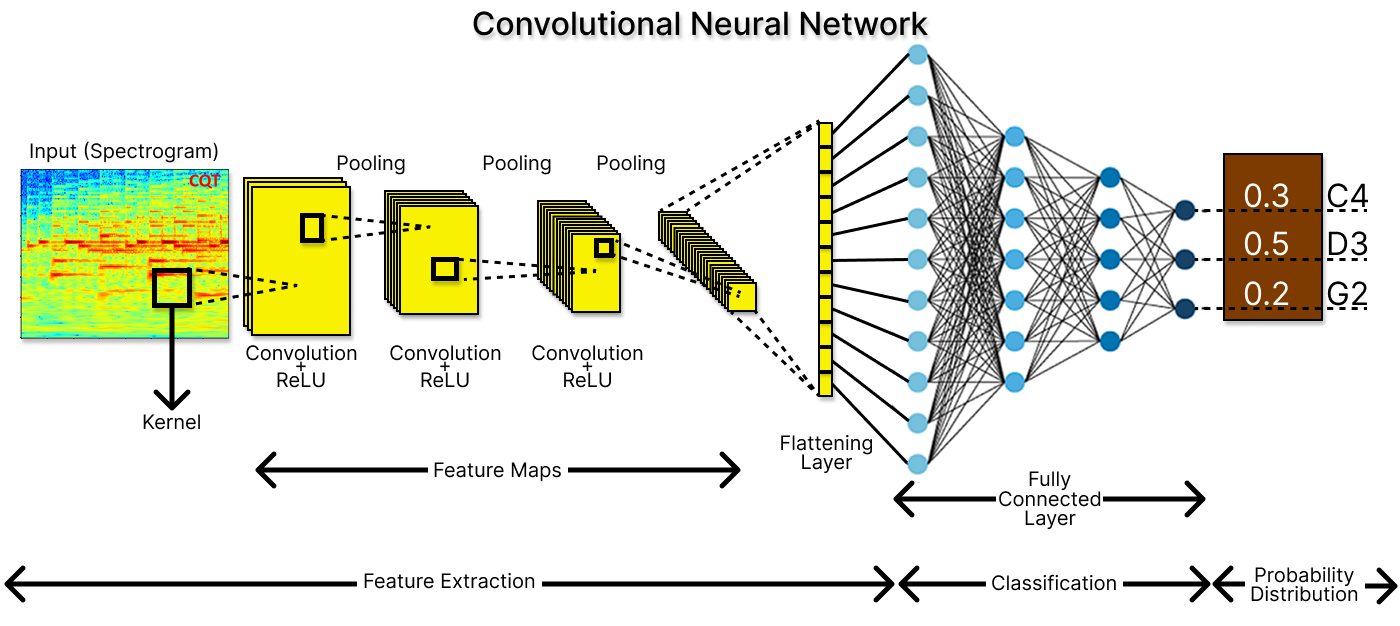
\includegraphics[width=1\textwidth]{Graphics/CNN}
    \caption[CNN Struktur]{Visualisierung einer CNN Struktur zur automatischen Musiktranskription. Eigene Darstellung in Anlehnung an  \cite{shahriar2020cnn}.}
    \label{fig:cnn-amt}
\end{figure}

Üblicherweise schließt sich, in einem AMT-System, nach einem CNN ein RNN an.
Dieses kann jedoch nur 1D-Vektoren verarbeiten und nicht einen 3D-Tensor.
Dieser 3D-Tensor wird deshalb vor der Übergabe durch eine Flattening-Operation
zeitschrittweise in 1D-Vektoren umgewandelt.
Dabei wird der Vektor mit einer Dimension von F × C erhalten.
Diese Vektoren werden dann an das folgende RNN weitergeleitet.

\subsubsection{Geschichtliche Einordnung von CNNs}
CNNs finden ihren Ursprung im Jahre 1979.
Die erste Architektur für CNNs wurde, unter dem Namen \enquote{Neocognitron}, veröffentlicht \cite{fukushima1980neocognitron}.
Das Neocognitron kann zwar als Vorläufer moderner Convolutional Neural Networks betrachtet werden,
unterschied sich jedoch wesentlich von späteren CNN-Architekturen.
Es dauerte weitere 10 Jahre bis das erste vollwertige Convolutional Neural Network veröffentlicht wurde \cite{lecun1989backpropagation}.
Dieses CNN Modell unterscheidet sich speziell in drei bestimmten Punkten zu dem Vorgänger Neocognitron.
LeCun integriert in seinem CNN Gradientenlernen durch Backpropagation,
wodurch das gesamte Netzwerk erstmals auf ein gemeinsames Ziel zu trainieren konnte.
Neocognitron besaß zudem, im Gegensatz zu LeCuns CNN,
keine Gewichtsverteilung mithilfe von Filtern, wie es in heutigen CNN Modellen Standard ist.
Das Neocognitron hatte zudem keine praktische Anwendung.
Es stellte zwar ein theoretisch wegweisendes Architekturkonzept dar,
doch die damaligen technischen Rahmenbedingungen erschwerten eine praktische Umsetzung.
Für AMT-Systeme wurden CNNs erst etwa ab dem Jahre 2015 relevant \cite{sigtia2016end}.
In dieser Arbeit wurden erstmals polyphone Musikstücke mithilfe von CNNs und weiteren KI-Modelle, transkribiert.
Seitdem sind CNNs ein wichtiger Bestandteil der modernen automatischen Musiktranskription.

\subsection{Recurrent Neural Networks}
RNNs sind neuronale Netze, welche entworfen wurden um Daten mit zeitlicher Struktur zu verarbeiten.
Dabei ist die Besonderheit von RNNs das diese ein Gedächtnis haben.
Wenn in einem AMT-System eine bestimmte Tonabfolge gespielt wurde,
kann sich das RNN diese merken und dementsprechend die fortlaufenden Ausgaben anpassen.
Dies passiert dank den Hidden States.
Diese stellen das Gedächtnis des RNNs dar und sind einer der wichtigsten Faktoren in einem RNN\@.
Die Hidden States werde im nächsten Abschnitt ausführlicher beschrieben.
Dieses Prinzip ist in der Musiktranskription sehr hilfreich,
da jede Note stark von den vorherigen gespielten Noten abhängt.
Takt, Rhythmus, Harmonie und die Melodie eines Musikstückes sind alles gute Beispiele,
warum diese sequenzielle Abfolge so passend in AMT-Systemen ist.

RNNs haben in der automatischen Musiktranskription mehrere Aufgabenfelder.
Je nachdem wie das RNN trainiert wird, bewältigt dieses alle Aufgaben oder nur einen Teil.
Diese Aufgaben bestehen aus Frame-Glättung (Temporal smoothing), Kontext-Modellierung (Temporal context modeling),
Feature-Zusammenführung (Sequential integration of acoustic features)
und Ausgabevorbereitung (time-distributed output classification).
Diese Aufgaben werden auf jedes Zeitfenster, auf jeden 1D-Vektor des CNNs, angewendet.
Doch bevor der Fokus auf diese einzelnen Aufgaben gelegt werden kann, muss zunächst geklärt werden, was Hidden States sind.

\begin{description}[style=nextline]
\item[Hidden States]\label{itm:hidden}
Hidden States sind das grundlegende Prinzip, warum RNNs funktioniere.
Sie stellen das Gedächtnis des RNNs dar und helfen somit
anderen Modulen Vorhersagen über bestimmte musikalische Eigenschaften zu treffen.
Für jeden 1D-Vektor, den das CNN liefert, wird ein Hidden State erstellt.
Diese werden sequenziell, mit Abhängigkeit zum vorherigen Hidden States, definiert.

Die folgende Gleichung beschreibt, wie der aktuelle Hidden State $h_t$ aus dem Eingabevektor $x_t$ und dem vorherigen Hidden State $h_{t-1}$ berechnet wird.
Der vorherige Hidden State $h_{t-1}$ repräsentiert nicht nur den unmittelbar vorausgehenden Zustand,
sondern auch alle davorliegenden, da diese in die Berechnung jedes neuen Hidden States einfließen.
Die Funktion $f$ repräsentiert dabei eine nichtlineare Transformation, mithilfe der Gewichte des RNNs.
Somit wird sichergestellt, dass der neue Hidden State sowohl den aktuellen Eingabevektor $x_t$, als auch die vorherigen Hidden States $h_{t-1}$ berücksichtigt.
\[
\mathbf{h}_t = f(\mathbf{x}_t, \mathbf{h}_{t-1})
\]

Hidden States enthalten das Wissen der vorherigen Zeitfenster über zeitliche Muster, wie Sustain und Akkordstruktur.
Alleine können Hidden States keine eigene Entscheidung über bestimmte Noten fallen.
Dafür müssen andere Module die Informationen der Hidden States später richtig verwerten.
Jeder Hidden State hat eine Anzahl von Dimensionen, welche gleich der Anzahl der Neuronen im RNN ist.
\end{description}

\subsubsection{Grundstruktur eines RNNs}
Bei der Frame-Glättung bekommt das RNN als Input die Aktivierungswerte des Zeitfensters.
Es betrachtet diese mit Kontext zu den vorherigen Zeitfenstern, um falsche Vorhersagen auszuschließen.
Das CNN hat dem RNN schon Vorhersagen für bestimmte Noten gegeben.
Diese Vorhersagen könnten jedoch Fehler enthalten.
Zum Beispiel kann die Note C4 für den Frame 6 und 8 aktiv sein,
aber bei dem Frame 7 hat das CNN diese Note nicht als aktiv angesehen.
Es ist sehr unwahrscheinlich, das eine Note für nur einen Frame ausfällt.
Solche Arten von Fehlern verarbeitet das RNN über mehrere Zeitfenster hinweg, mithilfe seiner wiederkehrenden Struktur.
Dieser Vorgang wird auch als zeitliche Entfaltung bezeichnet.
Deshalb aktiviert das RNN den Ton C4 auch im Frame 7.

Die folgende Abbildung zeigt die Entfaltung eines einzigen RNN-Blocks über mehrere Zeitpunkte hinweg.
In der Abbildung steht $x$ für den 1D-Inputvektor eines CNNs,
$h$ für den Hidden State und dem somit verbundenen Gedächtnis des RNNs
und $o$ für den Outputvektor, mit dem weiter gerechnet wird.
Die Buchstaben $W$, $U$ und $V$ stellen dabei die verschiedenen
Gewichte \enquote{Input-Weight}, \enquote{Recurrent-Weight} und \enquote{Output-Weight} dar.
\begin{figure}[H]
    \centering
    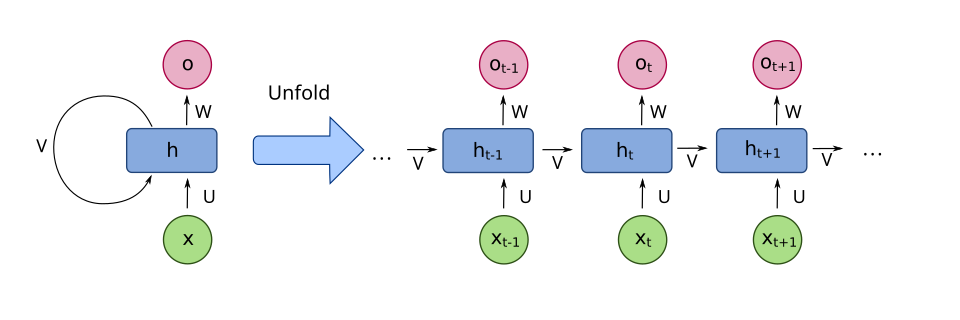
\includegraphics[width=1\textwidth]{Graphics/rnn_unfold}
    \caption[Entfaltung eines RNN-Blocks]{Entfaltung eines RNN-Blocks  \cite{wikimediaRNN}.}
    \label{fig:rnn_block_unfold}
\end{figure}
Diese Abbildung illustriert folgende Formel.
Dabei steht $b$ für den Bias-Vektor des Hidden Layers und $c$ für den Bias-Vektor des Output-Layers.
\begin{align*}
h_t &= \tanh\left( W \cdot x_t + U \cdot h_{t-1} + b \right) \\
o_t &= \sigma\left( V \cdot h_t + c \right)
\end{align*}

Neben der Frame-Glättung wird die Kontext-Modellierung auf den gegebenen Input angewendet.
Als Input bekommt diese auch die 1D-Vektoren des CNNs.
In der Kontext-Modellierung werden größere zeitliche Zusammenhänge betrachtet.
So kann die Kontext-Modellierung, mithilfe des Hidden States,
den Notenverlauf oder auch die Länge einer Note vorhersehen.
Je nach den Trainingsdaten ist es zum Beispiel üblicher das auf C4 ein D3 folgt,
was durch die Kontext-Modellierung angepasst wird.
Dieser musikalische Kontext ist aber immer stark von der Musikrichtung und von den Musikern abhängig,
welche in den Trainingsdaten vorhanden sind.
Bei Jazz und Pop oder Johann Sebastian Bach und Taylor Swift unterscheidet sich der Stil der Tonabfolge extremst.
Zudem wird Onset, Sustain und Offset stabilisiert.
Durch vorherige Beispiele weiß die Kontext-Modellierung,
wie lange eine bestimmte Note andauern wird und kann so das Offset der Note einschätzen.
Als Output entstehen kontextabhängige Vektoren.
Sie haben die gleiche Struktur wie die 1D-Vektoren vom CNN, sind aber entsprechend dem Kontext angepasst.

Die Feature-Zusammenführung ist der letzte wichtige interne Schritt eines RNNs.
Bei diesem werden aus lokalen alleinstehenden Informationen eines Zeitfensters, konkrete musikalische Ereignisse.
Dadurch schreibt das RNN Ereignisse wie Akkorde, Noten, Onsets und weitere heraus.
Dafür muss die Feature-Zusammenführung sich die einzelnen 1D-Vektoren als eine Folge von Events anschauen.
Dies passiert über den Hidden State.
Das wird vor allem wichtig, wenn später eine MIDI-Datei ausgegeben werden soll,
da in dieser auch die einzelnen musikalischen Ereignisse aufgeschrieben sind.
Als Output entstehen kontextreiche Vektoren.
Diese Vektoren sind, durch die vorherigen Module angepasste und verbesserte, Hidden States.

Die Ausgabevorbereitung ist der letzte Schritt des RNNs,
wodurch nun die gesammelten Daten zu echten musikalischen Ereignissen zusammengefügt werden.
Als Input werden die, durch die Feature-Zusammenführung verbesserten, Hidden States genutzt.
Zunächst werden diese durch ein Fully Connected Layer geschickt.

Ein Fully Connected Layer ist ein Klassifikator, welcher den Hidden States auf eine gewünschte Dimension bringt.
Wenn zum Beispiel Klaviertasten vorhergesagt werden sollen, werden alle Hidden States mit 88 Dimensionen ausgestattet.
Bei MIDI-Dateien wären es 128 Dimensionen.
Die Werte, welche aus dem Fully Connected Layer stammen, sind jetzt noch nicht richtig interpretierbar.
Um diese als konkrete und normalisierte Wahrscheinlichkeiten darstellen zu können,
wird eine Aktivierungsfunktion eingesetzt.
Mit beispielsweise der Sigmoid-Funktion als Aktivierungsfunktion
können alle Werte normiert in einem Bereich zwischen 0 und 1 gebracht werden.
Sagen wir, wir wollen jetzt die gespielten Klaviertasten vorhersagen.
Dann hat jeder Hidden State für alle Klaviertasten einen eigenen Wert mit einer Wahrscheinlichkeit,
dass diese Taste zu dem gewählten Moment gespielt wurde.
Zum Schluss muss jetzt ein Threshold bestimmt werden.
In polyphonen Musikstücken können immer mehrere Noten gleichzeitig erklingen,
weshalb nicht einfach die Note mit der höchsten Wahrscheinlichkeit ausgewählt werden kann.
Deshalb wird ein Threshold genutzt, zum Beispiel bei 50\%,
welcher bestimmt, wie viel Prozent eine Note braucht, um als aktiv zu gelten.
Durch Postprocessing können einige Eigenschaften wie Rauschen noch herausgefiltert werden.
Postprocessing ist jedoch nicht relevant für den KI-Ablauf.
Wenn das Ergebnis zufriedenstellend ist, kann es in das gewünschte Output-Format,
standardmäßig MIDI-Dateien, eingefügt werden.

Heutzutage sind RNNs nur die grundlegende Struktur.
Basierend auf dieser gibt es einige verbesserte Systeme,
welche Aktiv in AMT-Systemen und anderen KI-Systemen genutzt werden.
Zwei dieser Systeme sind Long Short-Term Memory's (LSTM) und Bidirektionale RNNs (BiRNN).
Diese werden im folgendem Abschnitt ausführlicher erklärt.

\subsubsection{Long Short-Term Memory}
LSTMs sind verbesserte RNNs.
Diese kontrollieren durch Gates besser, welche Daten sie wirklich in den Hidden State speichern möchten.
Dadurch lässt sich das neuronale Netz noch weiter an die gewünschten Ansprüche anpassen.

In einem einfachen RNN werden alle Daten, egal ob sinnvoll oder nicht, miteinander in dem Hidden State kombiniert.
Somit kann sich das RNN langfristig schwieriger Information merken.
Wenn zum Beispiel im 2.\ Hidden State ein Onset erkannt wurde, kann der 20.\ Hidden State
sich das schlechter merken, da viele andere Informationen mitgeschrieben wurden.
LSTMs lösen dieses Problem mit Forget, Input und Output Gates und dem Cell State.
Der Cell State stellt das Langzeitgedächtnis des LSTMs dar.
Er berechnet sich aus den drei Gates.
Das Forget Gate bestimmt, welche Informationen aus dem vorherigen Cell State gelöscht werden sollen.
Das Input Gate bestimmt, welche neuen Inhalte aus dem neuen Zeitfenster aufgenommen werden.
Dabei ist der Cell-candidate die Datenmenge, welche zum Speichern, durch das Input Gate, vorgeschlagen wird.
Das Output Gate bestimmt, welcher Teil des Cell States zu dem neuen Hidden State hinzugefügt wird.
\begin{align*}
f_t &= \sigma(W_f x_t + U_f h_{t-1} + b_f) \quad &&\text{(Forget Gate)} \\
i_t &= \sigma(W_i x_t + U_i h_{t-1} + b_i) \quad &&\text{(Input Gate)} \\
o_t &= \sigma(W_o x_t + U_o h_{t-1} + b_o) \quad &&\text{(Output Gate)} \\
\tilde{c}_t &= \tanh(W_c x_t + U_c h_{t-1} + b_c) \quad &&\text{(Cell-candidate)} \\
c_t &= f_t \odot c_{t-1} + i_t \odot \tilde{c}_t \quad &&\text{(Cell State)} \\
h_t &= o_t \odot \tanh(c_t) \quad &&\text{(Aktueller Hidden State)}
\end{align*}
Dadurch kann sich ein LSTM die verschiedenen musikalischen Ereignisse,
über das gesamte Audiosignal, besser im Zusammenhang merken.

Folgende Abbildung zeigt einen Zeitschritt in einem LSTM.
Dabei sind die Komponenten gleich benannt wie in der Abbildung-\pref{fig:rnn_block_unfold}.
Das $c$ steht für den Cell-State.
Intern in der \enquote{LSTM Unit} stehen die Buchstaben $F$, $I$ und $O$ für die Gates:
\enquote{Forget Gate, Input Gate und Output Gate}.
\begin{figure}[H]
    \centering
    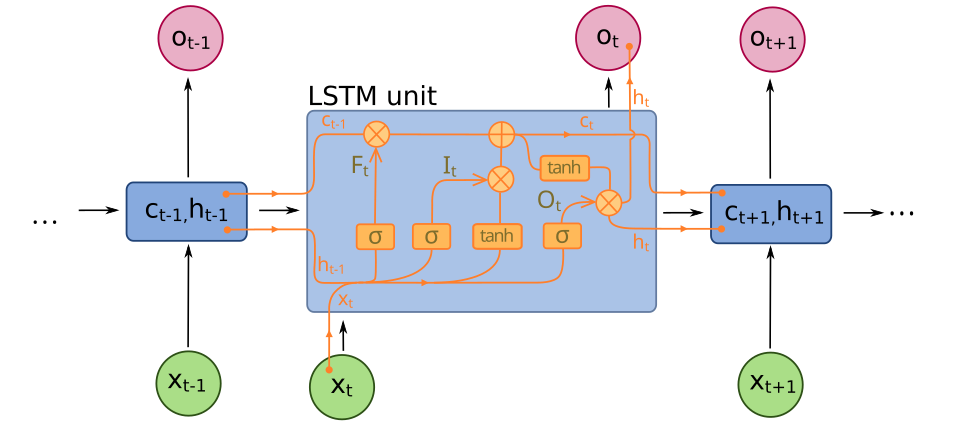
\includegraphics[width=1\textwidth]{Graphics/LSTM_timestep}
    \caption[LSTM Zeitschritt]{Zeitschritt eines LSTMs  \cite{wikimediaRNN}.}
    \label{fig:lstm_timestep}
\end{figure}

\subsubsection{Gated Recurrent Units}
GRUs sind, neben LSTMs, eine weitere spezielle Art von RNNs \cite{chung2014empirical}.
Sie wurden erfunden, um bestimmte Probleme von RNNs zu lösen.
Insbesondere das Problem des \enquote{Vanishing Gradients} sollten GRUs lösen.
GRUs steuern mithilfe von Gates, welche Informationen gemerkt und welche vergessen werden sollen.
Sie sind, im Gegensatz zu LSTMs, eher für kleinere Aufgaben geeignet.
Dafür sind sie weniger fehleranfällig und haben ein schnelleres Training.

Ein GRU besitzt zwei Gates.
Sie haben, genau wie bei LSTMs, die Aufgabe das Gedächtnis des KI-Models zu verwalten.
Das Reset Gate schaut sich den alten Hidden State an und entscheidet,
wie viel von diesem Wissen in den neuen Hidden State mit einfließt.
Das Update Gate hingegen sieht den aktuellen Hidden State und überlegt,
welche Informationen davon in das Langzeitgedächtnis mit einbezogen werden.
Danach führt das Update Gate die beiden überarbeiteten Hidden States zusammen zum neuen Hidden State.

Das Problem des Vanishing Gradients betrifft das Gedächtnis neuronaler Netze und tritt insbesondere während der Trainingsphase auf.
Bei der Backpropagation werden die Gradienten mit jedem durchlaufenen Layer kleiner, sodass betroffene Layer im Netzwerk kaum noch dazulernen.
Dies liegt daran, dass Aktivierungsfunktionen Werte im Bereich zwischen 0 und 1 zurückgeben und ihre Ableitungen ebenfalls kleiner als 1 sind.
Da die Gradienten bei jedem Schritt mit diesen Ableitungen multipliziert werden, schrumpfen sie exponentiell mit zunehmender Netzwerktiefe.
Infolgedessen verliert das Modell die Fähigkeit, Informationen über längere Zeiträume hinweg zu speichern.
Bei GRUs wird das Problem des Vanishing Gradients durch die Gates gelöst.
Sie stellen eine gewichtete Mischung aus altem und neuem Hidden State dar.
Dadurch wird der Gradient nicht ständig verkleinert
und wichtige Informationen können über einen langen Zeitraum gespeichert werden.

Folgende Abbildung zeigt einen Zeitschritt in einem GRU.
Die Komponenten sind gleich benannt wie in der Abbildung-\pref{fig:rnn_block_unfold}.
Intern in der \enquote{GRU Unit} stehen die Buchstaben \enquote{R und Z} für die Gates:
\enquote{Reset Gate und Update Gate}.
\begin{figure}[H]
    \centering
    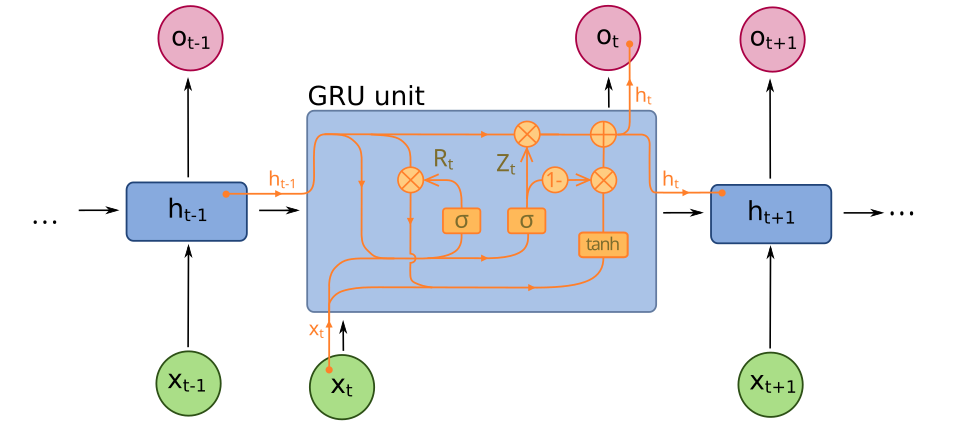
\includegraphics[width=1\textwidth]{Graphics/GRU_timestep}
    \caption[GRU Zeitschritt]{Zeitschritt eines GRUs  \cite{wikimediaRNN}.}
    \label{fig:gru_timestep}
\end{figure}

\subsubsection{Bidirektionale RNNs}
Um ein noch besseres Ergebnis zu erhalten, kann auch ein bidirektionales RNN genutzt werden.
Dieses besteht aus zwei RNNs.
Eines liest die Zeitfenster von vorne und das andere von hinten ab.
Dadurch entsteht die doppelte Menge an Hidden States und die gesamte Vorhersage wird robuster.

Die folgende Formel beschreibt die Konstruktion des Hidden States $\mathbf{h}_t$ in einem bidirektionalen RNN.
Dabei setzt der neue Hidden State sich aus zwei Teilen zusammen.
Dem Vorwärts-Hidden-State $\overrightarrow{\mathbf{h}}_t$,
der die Informationen aus der Vergangenheit bis zum Zeitpunkt $t$ enthält,
und dem Rückwärts-Hidden-State $\overleftarrow{\mathbf{h}}_t$,
der die Informationen aus der Zukunft bis $t$ einbezieht.
Diese beiden Hidden States werden zusammengefügt,
sodass der gewonnene Hidden State Informationen über das gesamte Musikstück enthält.
\[
\mathbf{h}_t = \left[ \overrightarrow{\mathbf{h}}_t \ ;\ \overleftarrow{\mathbf{h}}_t \right]
\]

Auch in AMT-Systemen sind bidirektionale RNNs sehr hilfreich,
da musikalische Ereignisse auch eine klar verständliche Abhängigkeit von der Zukunft in die Vergangenheit haben.
Das gleiche Prinzip lässt sich auch auf LSTMs oder GRUs anwenden,
sodass beispielsweise ein bidirektionales LSTM entsteht.
Bidirektionale RNNs sind noch robuster, aber dafür ist der Rechenaufwand bei weitem höher.
Ein bidirektionales RNN findet sich auch in folgender Arbeit \cite{hawthorne2017onsets}.

\subsubsection{Geschichte und Weiterentwicklung von RNNs und ihren Varianten}
Die Geschichte von Recurrent neural networks reicht bis in das Jahr 1990 zurück \cite{elman1990finding}.
In dieser Arbeit wurde erstmals die Idee der Rückkopplung eingebaut,
wodurch der Output eines Neurons als zusätzliche Eingabe im nächsten Zeitfenster genutzt wird.
Das resultierte später in den Hidden States.
Diese Arbeit baute den Grundstein für alle weiterführenden RNNs.
Ein weiterer früher Ansatz wurde bereits 1986 als technischer Bericht vorgestellt und 1997 publiziert \cite{jordan1997serial}.
Er führte sogenannte Kontexteinheiten ein, bei denen der Output eines Neurons in das folgende Zeitfenster rückgekoppelt wird.
Damit wurde ein alternativer Mechanismus zur Sequenzmodellierung vorgeschlagen,
der sich von Elmans Rückkopplung aus dem Hidden Layer unterschied und wichtige Grundlagen für spätere Varianten von RNNs schuf.
Zudem wurde, im Jahre 1997, das erste Bidirektionale RNN \cite{schuster1997bidirectional}
und das erste LSTM erfunden \cite{hochreiter1997long}.
Erst über ein Jahrzehnt später wurde das erste GRU entwickelt \cite{chung2014empirical}.
RNNs fanden ihren Weg in die automatische Musiktranskription, fast zeitgleich zu CNNs, im Jahre 2015 \cite{sigtia2015hybrid}.
Für LSTMs dauerte die Einbindung in AMT-Systeme etwas länger.
Erst im Jahre 2016 wurde ein LSTM in einem AMT-System eingefügt \cite{sigtia2016end}.
Dahingegen wurde das erste Bidirektionale RNN erst Ende 2017 in ein AMT-System integriert \cite{hawthorne2017onsets}.
Noch ein Jahr später wurde das erste Mal auch ein GRU in einem AMT-System genutzt \cite{jung2018adaptive}.

\subsection{Transformers}
Transformer sind eine, von Google entwickelte Deep-Learning Architektur \cite{vaswani2017attention},
die mit dem Prinzip der Self-Attention, zur natürliche Sprachverarbeitung genutzt wird.
Auch Transformer verarbeiten die Daten, wie ein LSTM, sequentiell.
Jedoch wurde zu dieser Verarbeitung noch der Attentionmechanismus hinzugefügt,
welcher der grundlegende Baustein eines Transformer-Modells ist.
Die Architektur eines Transformers besteht grundlegend aus drei Bausteinen.
Diese sind Input Embedding mit Position Encoding, Self-Attention Layer und Feedforward Layer.
Input Embedding und Position Encoding werden nur einmalig am Anfang des Transformers durchgeführt.
Dahingegen werden Self-Attention und Feedforward mehrmals hintereinander aufgerufen.
Dies passiert grundsätzlich 6-, 12- oder 24-mal, wodurch das Transformer-Modell an Layern gewinnt.
Dieser Schritt wird so oft wiederholt, damit der Transformer immer komplexere musikalische Strukturen erkennen kann.
Als Nächstes werden die einzelnen Schritte eines Transformers näher erläutert.

\subsubsection{Input Embedding und Position Encoding}
Zunächst müssen die Daten, welche der Transformer verarbeiten soll in das richtige Format für diesen umgewandelt werden.
Dafür ist das Input Embedding zuständig.
Tokens sind einzelne Datenpunkte wie beispielsweise kurze Wörter wie \enquote{hallo}.
Wenn zum Beispiel bei ChatGPT die Anfrage \enquote{Wie alt sind die Planeten unseres Sonnensystems} gestellt wird,
dann wird zwar das Wort \enquote{alt} als ein Token gespeichert, aber längere Wörter wie \enquote{Sonnensystem}
werden aufgeteilt in \enquote{Sonn} und \enquote{ensystem}.
Je nach Tokenizer-Version, die der jeweilige Transformer nutzt, kann dies jedoch abweichen.
Bei diesem Beispielsatz werden, alleine für die Wörter, neun Tokens genutzt.
Tokens können auch einzelne Satzzeichen oder Symbole sein.
Für verschiedene Transformer Modelle gibt es immer eine maximale Tokenanzahl,
bei GPT-3.5 sind es zum Beispiel ungefähr 4000 Tokens.
Diese Tokens sind für den Input und Output.
Heißt, wenn der Input zu viele Tokens nutzt, gibt es weniger Tokens für den Output.
Dies ist jedoch häufig, wie an der Menge der Tokens für unseren Beispielsatz zu sehen ist, kein größeres Problem.
In AMT-Systemen stellen Tokens Zeitfenster (Frames) oder Musik-Events (Onsets etc.) dar.
Jedoch können diese von einem Transformer nicht verarbeitet werden,
weshalb sie durch Input Embedding erstmals in Vektoren umgewandelt werden.
Dies passiert über eine Embedding-Matrix, welche die einzelnen Tokens in den Vektorraum einbettet.
\[
\displaystyle
\text{Embedding-Matrix} \in \mathbb{R}^{\left( \text{Maximale Tokenanzahl } \times \text{ Embedding-Dimension} \right)}
\]
Tokens, welche ähnliche musikalische Eigenschaften speichern, werden im Vektorraum näher beieinander gespeichert.
Das Modell kann die Tokens, durch die gesammelten Daten im Training, richtig einordnen.

Nun sieht der Transformer die Tokens trotzdem nur als zahlreiche Vektoren, ohne Rheinfolge, an.
Um den Tokens einen Sinn zu geben, müssen diese eine explizite Position erhalten.
Das wird durch Position Encoding gemacht.
Durch Sinus- und Cosinunsfunktionen wird für jeden Token ein eindeutiger Positionsvektor berechnet.
Dies geschieht, indem für jede Dimension, die unsere Tokens besitzen, eine Funktion mit unterschiedlicher Frequenz gebildet wird.
Bei geraden Dimensionen wird eine Sinusfunktion genutzt und bei ungeraden eine Cosinusfunktion.
So erhält jede Position einen eindeutigen Positionsvektor,
während nahe Positionen ähnliche Encodings und somit geringeren Abstand zueinander besitzen.
Dadurch kann der Transformer die relative Position, verschiedener Tokens,
gut miteinander vergleichen und zugleich wiederkehrende Muster erkennen.
Danach wird der Positionsvektor dem Tokenvektor aufaddiert.
Moderne Transformer besitzen manchmal auch gelernte Position Embeddings,
wodurch die Positionen schon durch das Training bekannt sind.
Diese Vektoren werden, als Input, weiter an den Transformer geleitet.

\subsubsection{Self-Attention Layer}
Jeder Input-Vektor wird einzeln behandelt.
Durch Self-Attention kann sich jeder Vektor merken, welche anderen Vektoren für ihn relevant sind.
Zunächst wird jeder Input-Vektor in drei verschiedene Vektoren umgewandelt.
Diese Vektoren heißen \enquote{Query}, \enquote{Key} und \enquote{Value}.
\begin{itemize}
  \item \textbf{Query ($Q$)}: Bestimmt, auf welche Informationen aus anderen Tokens das Modell aktuell achten möchte.
  \item \textbf{Key ($K$)}: Zeigt anderen Tokens, was dieser Input-Vektor anderen Tokens, für Informationen, anbieten kann.
  \item \textbf{Value ($V$)}: Enthält die tatsächlichen Informationen des Input-Vektors.
\end{itemize}
Als Nächstes wird der \enquote{Attention Score} berechnet.
Durch diesen wird die Kompatibilität zu anderen Tokens berechnet.
Mit Kompatibilität ist dabei die Ähnlichkeit zwischen einem Query- und einem Key-Vektor gemeint.
Diese gibt an, wie stark ein Token im Verhältnis zu einem anderen berücksichtigt werden soll.
Als Ergebnis entsteht für jeden Token eine Matrix.
Jeder Wert in dieser Matrix steht für die Ähnlichkeit zwischen zwei verschiedenen Tokens.
Diese Werte sind die Attention Weights.
Durch Softmax werden diese Werte normalisiert.
Als Letztes werden diese Attention Weights mit den Value-Vektoren verbunden.
\[
\text{Output} = \text{Attention Weights} \times \text{Value Vektoren}
\]
Nun können die einzelnen Tokens sich besser auf die Tokens fokussieren, welche wirklich wichtig für deren Ergebnis sind.

\subsubsection{Feedforward Layer}
Der Feedforward Layer stammt von der Idee eines \enquote{Feedforward Neural Networks} (FNN).
Dieses neuronale Netz verläuft immer nur in eine Richtung und hat keine Rückkopplung.
Das heißt jeder Token wird für sich alleine, nacheinander, umgeschrieben.
Das funktioniert, da die jeweilige Gewichtung schon im Self-Attention Layer stattgefunden hat.
Im Feedforward Layer passiert dann folgendes.
Zunächst werden die Vektoren, welche aus dem Self-Attention Layer stammen,
mit einer Gewichtsmatrix auf eine höhere Dimension transformiert.
Durch die Erhöhung der Dimension bekommt das Netzwerk mehr Freiraum Informationen voneinander zu trennen
und komplexere Zusammenhänge zu modellieren.
Durch eine Aktivierungsfunktion, zum Beispiel ReLU, erlernt das Modell jetzt nichtlineare Abhängigkeiten.
Diese Aktivierungsfunktion gehört zu dem Hidden Layer des FNN.
Ein FNN kann mehrere Hidden Layer besitzen, welche alle die Input-Werte in irgendeiner Form verändern.
Als Nächstes wird der Vektor wieder auf seine ursprüngliche Dimension zurückprojiziert,
wodurch nur die wichtigsten Informationen erhalten bleiben.
Mathematisch sieht der Feedforward Layer folgendermaßen aus:
\[
y_t = \text{FFN}(x_t) = \left( x_t W_1 + b_1 \right) \xrightarrow{\text{ReLU}} W_2 + b_2
\]
\begin{itemize}
  \item $x_t$: Eingabevektor des Tokens.
  \item $W_1, W_2$: Gewichtsmatrizen, zuständig für Dimensionserweiterung und -reduktion.
  \item $b_1, b_2$: Bias-Vektoren der jeweiligen linearen Projektionen.
  \item $\left( x_t W_1 + b_1 \right)$: Ergebnis der ersten linearen Projektion.
  \item $\text{ReLU}$: Aktivierungsfunktion zur Einführung von Nichtlinearität.
  \item $y_t$: Ausgabewert des Feedforward Layers für das Token.
\end{itemize}

\subsubsection{Geschichtliche Einordnung von Transformern}
Das erste Transformer-Modell wurde im Jahre 2017 erfunden \cite{vaswani2017attention}.
Durch den Self-Attention Layer wurde die sequenzielle Modellierung von Daten revolutioniert.
Es dauerte noch lange bis der erste Transformer auch in AMT-Systemen genutzt wurde.
Das liegt an mehreren Gründen.
Einerseits gibt es im Gegensatz zu natürlichen Sprachverarbeitung weniger Datensätze, von denen die Modelle lernen könnten.
Transformer trainieren auf einem globalen Level und brauchen daher eine große Menge an Datensätzen.
Die Rechenkosten von Transformer Modellen sind auch weitaus höher als bei anderen Systemen, wie CNNs und RNNs.
Zudem lag der Fokus bei AMT-Systemen für eine sehr lange Zeit überwiegend bei CNN und RNN basierenden Systemen,
da diese Anwendungsfälle bekannter waren in AMT-Systemen.
Das größte Problem war jedoch wahrscheinlich die Anpassung.
Transformer Modelle waren einfach nicht dafür ausgelegt musikspezifische Daten zu verarbeiten.
In der Musiktranskription wird immer mit langen Sequenzen, ein gesamtes Musikstück, gearbeitet.
Spezielle Transformer Modelle für diesen Anwendungsfall mussten noch programmiert werden.
Die ersten Ansätze für Transformer in AMT-Systemen wurden zwischen den Jahren 2021 und 2023 erstellt.
Eines der ausschlaggebendsten Modelle war der Music Transcription Transformer MT3,
welcher vom Magenta-Team bei Google Brain erstmals im Jahre 2022 veröffentlicht wurde \cite{gardner2021mt3}.
Dieses spielt eine große Rolle in der Transformer-basierten automatischen Musiktranskription,
da es das erste weit verbreitete Multi-Task-Transkriptionsmodell ist.
Eine der Letzten bedeutenden Errungenschaften zu Transformern und Musiktranskription ist das
YourMT3+ Modell, indem die MT3-Architektur noch weiter verbessert wurde \cite{chang2024yourmt3+}.

\subsection{Potentielle KI-Modelle}
Bei der KI integration in AMT-Systemen werden überwiegend CNNs und RNNs oder Transformer Modelle wie MT3 verwendet.
Jedoch gibt es noch andere KI-Modelle, die in AMT-Systemen integriert werden können.
Diese gehen, bei der Musiktranskription, ganz anders vor als die vorgestellten Module.
Je nach KI übernehmen sie auch eine ganz andere Aufgabe.
Im folgenden Abschnitt werden einige von diesen, eher experimentellen, KIs vorgestellt.
Wir fangen dabei bei der am meisten erprobten KI an,
sodass die letzten KIs nur theoretisch, für die Musiktranskription, besprochen worden.

\subsubsection*{Variational Autoencoder}
Variational Autoencoder (VAE) ist ein KI-Modell, welches komplexe Daten in eine verdichtete Form überführt
und durch Wahrscheinlichkeiten bestimmte Muster vorhersagen kann \cite{kingma2019introduction}.
Dabei ist wichtig zu erwähnen das VAE kein alleinstehendes KI-Modell ist,
sondern eher als Zusatz gilt um bestimmte Bereiche zu verbessern.
In der Musiktranskription könnte ein VAE zum Beispiel bei der Mehrdeutigkeit von Musik helfen.
Wenn mehrere Instrumente spielen ist es schwer die genauen Noten herauszuschreiben.
Da VAEs, anders als CNNs oder RNNs, als Ausgabe keine eindeutigen Noten herausgeben,
sondern eine Wahrscheinlichkeit, könnte dies helfen die Entscheidung, welche Note gerade spielt, robuster zu gestalten.
Dadurch, dass VAEs nur eine wahrscheinliche Version der Musik aus den Daten extrahieren,
könnten damit auch kreative Variationen des Musikstückes gebildet werden.
Die Methode, welche in VAEs genutzt wird, fand Ihren Ursprung in folgendem Paper \cite{kingma2013auto}.

\subsubsection*{Graph Neural Network}
Graph Neural Network (GNN) ist ein KI-Modell, welches dazu dient Daten, mit Abhängigkeit voneinander, zu verarbeiten.
Diese Daten werden in einem Graphen aus Knoten und Kanten gespeichert.
Dabei hat jeder Knoten seine eigenen Daten, die er in jedem Rechenschritt mit seinen benachbarten Knoten austauscht.
Knoten sind benachbart, wenn sie durch Kanten verbunden sind.
Dadurch wird jeder Knoten im Netzwerk mit mehr Kontext ausgestattet.
Natürlich machen RNNs und Transformer etwas Ähnliches wie ein GNN, mit zum Beispiel Backpropagation.
Der Unterschied ist hier, das GNNs keine bestimmte Reihenfolge, wie Wissen weitergeleitet wird, haben.
Es ist ein anderer Ansatz harmonische Abhängigkeiten miteinander zu kombinieren \cite{wu2020comprehensive}.

\subsubsection*{Diffusion Model}
Diffusion Modelle arbeiten mit Rauschen.
Aus komplettem Rauschen bauen sie Schritt für Schritt ein Musikstück zusammen.
Dabei entscheiden sie pro Rechenschritt nur einen kleinen Teil des Musikstückes,
wodurch mehrdeutige Passagen in Musikstücken auch noch im späteren Transkriptionsprozess behandelt werden können.
In dem Projekt DiffRoll, aus dem Jahre 2022, wurde ein Diffusion Model auf ein AMT-System angewendet \cite{cheuk2022diffroll}.

\subsubsection*{Reinforcement Learning}
Reinforcement Learning benutzen ein Belohnungssystem, damit der Agent sich beim Training richtig anpasst.
Sobald der Agent ein bestimmtes Ziel erreicht oder eine Handlung ausführt, wird dieser dafür belohnt.
Die Agenten, welche am meisten Belohnungen erzielen, werden kopiert und in der nächsten Iteration eingesetzt,
bis ein Agent die gewünschte Aufgabe erfüllt.
Dieses Prinzip wird vor allem in Videospielen eingesetzt, wo es grundlegend eindeutige Ziele gibt.
In der Musiktranskription könnte dieses Prinzip folgendermaßen umgesetzt werden:
Der Agent erhält als Input eine Audiodatei.
Danach erzeugt er Noten nacheinander.
Durch eine andere KI oder vorgefertigte MIDI-Dateien steht ein Vergleichsdatensatz zur Verfügung.
Falls die gewählten Noten vom Agenten gleich dem Vergleichsdatensatz sind, bekommt der Agent Belohnungen.
So kann er sich selber musikalisches Wissen aneignen und Transkriptionen von anderen KIs nochmal korrekturlesen \cite{li2018music}.

\subsubsection*{Energy-Based Model}
Der letzte Ansatz ist ein Energy-Based Model (EBM).
Ein EBM arbeitet mit Energie anstatt von Wahrscheinlichkeiten \cite{lecun2006tutorial}.
Die verschiedenen Arten, wie das EBM das Musikstück transkribieren kann, haben alle jeweils ihre eigene Energie.
Dabei haben die besten Möglichkeiten immer die niedrigste Energie, wie bei dem Gradientenabstiegsverfahren.
Dies ist für AMT-Systeme interessant, da das EBM somit zahlreiche verschiedene Transkriptionsraten wählen könnte.
In mehr improvisierten Musikrichtungen, wie Jazz, bildet das eine größere Vielfalt.
Auch Musiktheorie lässt sich in das Modell einbauen,
wodurch aus einem Musikstück Unmengen an Remixen kreiert werden können.
Der Ansatz von EBMs in AMT-Systemen ist,
von den zusätzlich vorgestellten KI-Modellen, wahrscheinlich einer der Interessantesten.
Jedoch sind EBMs sowohl schwer zu trainieren, als auch sehr rechenintensiv.
AMT-Systeme sind ohnehin schon recht anspruchsvoll,
weshalb noch kein EBM-Modell in der automatischen Musiktranskription zum Einsatz kam.

 % offen
\section{KI-basierende AMT-Systeme im Vergleich}
Im Laufe der Forschung zu AMT-Systemen wurden schon einige verschiedenen Architekturen eingesetzt und verbessert.
Jedes neue System hat, unabhängig des KI-Modells, eine komplett eigene Struktur und vorgehensweise.
Im Verlauf dieser wissenschaftlichen Arbeit wurde die Geschichte von AMT-Systemen behandelt
und die wichtigsten Konzepte der automatischen Musiktranskription dargestellt.
Deshalb wird sich jetzt dieses Letzte große Kapitel um die state of the art AMT-Systeme handeln.
Dafür werden zwei verschiedene AMT-Systeme vor.
Diese sind das CNN + GRU basierte Omnizart und das Transformer-basierte MT3-Modell.
Diese nutzen unterschiedliche KI-Modelle.
Deren Architektur, sowie deren stärken und schwächen, werden in dem folgenden Kapiteln ausgiebig erläutern.

\subsection{Omnizart}
Zum einen haben wir Omnizart, welches CNNs und RNNs als KI-Modelle nutzt \cite{wu2021omnizart}.
Der Name Omnizart setzt sich aus den Wörtern Omni (alles) und Mozart zusammen,
da ihr Ziel darin liegt, so viele Arten von Musik wie möglich zu transkribieren.
Je nach Anwendungsfall werden verschiedene KIs benutzt.
Dabei ist der Aufbau dieser KIs meistens gleich.
Alle KI-Modelle bestehen aus einem CNN und einem bidirektionalen GRU.
Der Anwendungsfall, zum Beispiel Drums oder Melody, hat dabei nur Einfluss auf die Trainingsdaten und dem Output.
Omnizart ist ein Open-Source-Toolkit für AMT.
Dadurch kann man, je nach Bedarf, ein KI-Modell auswählen was perfekt auf eine bestimmte aufgabe ausgelegt wurde.
Omnizart findet ihren Ursprung im Jahre 2020 am Music and Culture Technology Lab, National Taiwan University.
Omnizart hat seit seiner Gründung keine ausschlaggebenden weiteren Technologien, in der richtung KI, hinzugefügt.
Dafür gibt es für jeden vertretenen Anwendungsfall verschiedene CNNs und RNNs und einen open source code,
welchen man gut zur eigenen Forschung an AMT-Systemen nutzen kann.

Omnizart ist ein modulares AMT-System, welches auf einer Deep-Learning-Architektur basiert.
Der Trainingssatz besteht aus CQT-Spektren.
Die KI-Modelle lernen dabei durch Supervised Learning.

Die Piepline von Omnizart kann man in drei Schritte aufteilen:

\begin{figure}[H]
    \vspace{1em}
        \begin{tikzpicture}[>=stealth, thick]

            \node[align=right] at (-3,0) (label1) {\textbf{Preprocessing} \\ \footnotesize (Signalaufbereitung)};
            \node[align=right] at (-3,-2) (label2) {\textbf{KI-Modell} \\ \footnotesize (Merkmalerkennung)};
            \node[align=right] at (-3,-4) (label3) {\textbf{Postprocessing} \\ \footnotesize (Ausgabeaufbereitung)};

            \node at (1,0) (audio) {Audiodatei};
            \node at (5,0) (prep) {Preprocessing};
            \node at (9,0) (cqt) {CQT-Berechnung};
            \node at (1,-2) (cnn) {CNN};
            \node at (5,-2) (gru) {GRU};
            \node at (9,-2) (dense) {Dense-Layer};
            \node at (1,-4) (post) {Post-Processing};
            \node at (8.5,-4) (output) {MIDI/CSV/JSON/TXT}

            \draw[->] (audio) -- (prep);
            \draw[->] (prep) -- (cqt);
            \draw[->] (cqt.south) -- ++(0,-0.6) -| (cnn);
            \draw[->] (cnn) -- (gru);
            \draw[->] (gru) -- (dense);
            \draw[->] (dense.south) -- ++(0,-0.6) -| (post);
            \draw[->] (post) -- (output);

        \end{tikzpicture}
    \vspace{1em}
    \label{fig:omnizart}
    \caption[Omnizart Pipeline]{Eigene Darstellung der Omnizart Pipeline}
\end{figure}

Der erste Schritt ist die Vorverarbeitung und Merkmalsextraktion (Preprocessing).
Dadurch wird die Inputaudiodatei in ein CQT-Spektrogramm umgewandelt.
Zunächst wird das gegebene Audiosignal durch folgende Methoden standardisiert:
\begin{enumerate}
    \item \textbf{Mono-Konvertierung:} Die KI benötigt keine räumlichen Informationen, weshalb der linke und rechte Kanal von Stereosignalen in ein Monosignal addiert werden.
    \item \textbf{Normalisierung:} Der Wechsel von zu großen und kleinen Amplituden kann die KI überfordern und ungenaue Ergebnisse liefern, weshalb das Audiosignal durch normalisierung auf einen einheitlichen Lautstärkebereich gebracht wird.
    \item \textbf{Resampling:} Unterschiedliche Abtastraten führen zu Verzerrung und Frequenzverschiebung, deshalb wird diese auf eine einheitliche Rate, passend zu dem genutzten Modul, gebracht.
    \item \textbf{Trimming:} Falls am Anfang oder Ende des Audiosignals Stille ist, wird diese durch Trimming entfernt, sodass das KI-Modell nicht unnötig verwirrt wird.
\end{enumerate}
Danach wird das standardisierte Audiosignal umgeformt zu einem CQT-Spektrogramm.
% CQT-Spektrogramm erklären und darauf verweisen

Im zweiten Schritt werden die KI-Modelle genutzt, um die Merkmale des Audiosignals vorherzusagen und zu extrahieren.
Die meisten AMT-Systeme, welche im Laufe dieser Arbeit vermerkt wurden, besitzen eine ähnliche Architektur wie Omnizart \cite{hawthorne2017onsets}.
Der Unterschied zu diesen AMT-Systemen ist das Omnizart, je nach Anwendungsfall, verschiedene Module nutzt.
Omnizarts Module sind:
\begin{itemize}
    \item \textbf{Chord:} Akkorderkennung
    \item \textbf{Drum:} Drum-Transkription
    \item \textbf{Melody:} Melodietranskription
    \item \textbf{Vocal:} Gesangsmelodietranskription
    \item \textbf{Piano:} Polyphone Klaviertranskription
    \item \textbf{Multi-Pitch:} Mehrstimmige Tonhöhenschätzung
    \item \textbf{Beat/Downbeat/Chord-Labelling:} Rhythmus, Takt \& Akkorde
\end{itemize}
Jedes Modul bekommt als Input ein CQT-Spektrogramm.
Dieses wird durch ein CNN verarbeitet, welches die Eigenschaften und Merkmale der Musik extrahiert.
Mit diesen Daten modelliert dann ein GRU die zeitliche Abhängigkeit.
Durch den Dense Layer werden die Ergebnisse des GRUs in zum Beispiel Onsets,
Beats und zahlreiche weitere musikalischen Attribute, umgewandelt.

Im dritten Schritt wird der Output der KI-Modelle nochmals aufbereitet.
Fehler werden zunächst durch folgende Methoden verbessert:
\begin{enumerate}
    \item \textbf{Noten-Segmentierung:} Wenn derselbe Ton in zwei nacheinander folgenden Frame ein Onset hat, wird der zweite Onset gelöscht und der Note hinzugefügt, sodass keine Notendopplungen entstehen.
    \item \textbf{Onset-Korrektur:} Falls ein Onset zeitlich nicht zur richtigen Zeit erfasst wurde, wird der Einschwingzeitpunkt des Onset an seinen Frame genau angepasst.
    \item \textbf{Thresholding:} Noten, die nicht einen bestimmten Wahrscheinlichkeits-Threshold überschreiten, werden aussortiert.
    \item \textbf{Quantisierung:} Je nach Taktstruktur können Noten zeitliche angepasst werden, sodass diese besser in zum Beispiel einen 3/4-Takt passen und das Stück rhythmischer ist.
\end{enumerate}
Je nach Modul, welches man gerade nutzt, werden nur paar oder alle dieser Methoden eingesetzt.
Auch deren Parameter unterscheiden sich je nach Modul.
So hat das Drums-Modul ein viel kleineren Schwellwert als das Melodien-Modul bei Thresholding.
Danach werden die Vorhersagen in vollständige Noten (Onset/Sustain/etc.)
zusammengefasst und in das gewünschte Format übertragen.
MIDI ist dabei das wichtigste Format, da dieses relevant für Musiksoftware ist,
es gibt aber auch noch drei andere Formate die, je nach Modul, ausgegeben werden.
Fast immer wird auch eine CSV-Datei ausgegeben.
Darin befinden sich die Transkriptionsdaten, welche zur Analyse oder Forschung genutzt werden können.
JSON-Dateien werden in den Chord- und Beat-Modulen ausgegeben.
Dies liegt daran, dass JSON-Dateien verschachteltet Daten, wie Akkordfolgen über mehrere Takte, besser speichern können.
In ihnen werden vor allem Takt-Informationen und Daten für Akkorde gespeichert.
TXT-Dateien werden dahingegen nur wahlweise in Modulen genutzt.
Sie sind ausschließlich für Debugging dar, weshalb sie für die meisten Nutzer nicht relevant sind.
Die Daten werden, in einer TXT-Datei, in einer unstrukturierten Liste ausgegeben.

\subsection{MT3}
Das Transformer-Modell, welches jetzt näher erläutert wird, heißt MT3.
MT3 steht für \enquote{Multi-Task Multitrack Music Transcription}.
MT3 ist gleichzeitig der Name für das Transformer-basierte KI-Modell, als auch für das überliegende AMT-System.
Diese beiden sind untrennbar voneinander, da sie zu einer End-to-End-Architektur gehören.
Das MT3-Modell bildet einen wichtigen Meilenstein für die Transformer-basierte automatische Musiktranskription.
MT3 ist das erste weit verbreitete Multi-Task-Transkriptionsmodell,
das heißt verschiedene Transkriptionsaufgaben werden von einem einzigen Modell gelöst.
Frühere Modelle brauchten zum Beispiel für Drums und die Melody,
wie es bei Omnizart der Fall ist, verschiedene KI-Modelle.
Durch die Communityversion YourMT3+ wird dieses KI-Modell immer weiter gepflegt und verbessert.

MT3 ist ein Transformer-Modell, welches spezifisch für Musiktranskription entwickelt wurde.
Es besteht grundlegend aus folgenden Bereichen:
\begin{figure}[H]
    \vspace{1em}
    \begin{tikzpicture}[>=stealth, thick]

        \node[align=right] at (-3,0) (label1) {\textbf{Preprocessing} \\ \footnotesize (Signalaufbereitung)};
        \node[align=right] at (-3,-2) (label2) {\textbf{KI-Modell} \\ \footnotesize (Transformer)};
        \node[align=right] at (-3,-4) (label3) {\textbf{Postprocessing} \\ \footnotesize (Token-Ausgabe)};

        \node at (0,0) (audio) {Audiodatei};
        \node at (3,0) (logmel) {Log-Mel-Spek.};
        \node at (6,0) (frames) {Frames};
        \node at (9,0) (projection) {Lineare Projektion};
        \node at (0,-2) (encoder) {Transformer Encoder};
        \node at (9,-2) (decoder) {Transformer Decoder};
        \node at (0,-4) (tokens) {Token-Sequenz};
        \node at (9,-4) (output) {MIDI};

        \draw[->] (audio) -- (logmel);
        \draw[->] (logmel) -- (frames);
        \draw[->] (frames) -- (projection);
        \draw[->] (projection.south) -- ++(0,-0.6) -| (encoder);
        \draw[->] (encoder) -- (decoder);
        \draw[->] (decoder.south) -- ++(0,-0.6) -| (tokens);
        \draw[->] (tokens) -- (output);

    \end{tikzpicture}
    \vspace{1em}

    \label{fig:mt3}
    \caption[MT3 Pipeline]{Eigene Darstellung der MT3 Pipeline}
\end{figure}

Als Input wird eine Audiodatei bereitgestellt.
Meistens geht man mit dem Datentyp WAV (Waveform Audio File Format), da dieser verlustfrei und standardisiert ist.
Das Audiosignal wird dann mit STFT analysiert und als Spektrogramm ausgegeben.
Mithilfe von Librosa wird aus diesem ein Log-Mel-Spektrogramm erzeugt.
Librosa ist ein Python Paket, welches wichtige Methoden für Musik und Audio analyse bereitstellt.
Dieses Log-Mel-Spektrogramm wird nun in Frames aufgeteilt.
In dem MT3-Modell sind diese Frames meist 32ms lang.
jeder Frame besitzt N Mel-Frequenzbänder, welche die Dimensionsgröße dieses Frames bestimmen.
Um jetzt für jeden Frame eine einheitliche Dimension zu bekommen,
mit der die KI Arbeiten kann, wird lineare Projektion genutzt.
Lineare Projektion ist ein Matrix-Multiplikator, welche ein Frame auf eine,
für das KI-Modell, normalisierte Dimension bringt, zum Beispiel 512 oder 1024.
Daraus entstehen Input Embeddings, mit denen die KI nun arbeiten kann.

Jetzt folgt der Encoder, welcher das normale Prinzip eines Transformers,
mit Self-Attention Layer und Feedforward Layer, ausführt.
In dem MT3-Modell werden, vor der ausführung der Layer,
die Positionen der Frames durch Positional Embeddings festgelegt.
In MT3 besteht der Encoder aus 6 vollständigen Transformer-Layern.
Der Inhalt jedes Frames wird jetzt zusammenhängen mit allen anderen Frames gesetzt.
Daraus resultieren Vektoren, welche kontextreiche Informationen des Musikstückes besitzen.
Diese Vektoren werden weiter an den Decoder geleitet

Aus den gegebenen Vektoren extrahiert der Decoder die wichtigen Daten.
Neben den Encoder Vektoren als Input bekommt dieser zudem autoregressive Tokens.
Autoregressive Tokens sind bereits generierte Tokens,
die im Training meist aus den echten Daten stammen (Teacher Forcing)
und beim Einsatz vom Modell selbst generiert werden.
Dadurch bekommt der Decoder mehr Kontext für die zu generierenden Tokens.
Neben den normalen Tokens bekommen auch die autoregressiven Tokens Positional Embeddings aufaddiert.
Bevor der Decoder nun durchläuft, kann man mithilfe von Task-Conditioning, einen Task-Token hinzufügen.
Das MT3-Modell transkribiert immer polyphon, jedoch kann man durch den Task-Token trotzdem den Output auf
einen bestimmten Task, wie zum Beispiel Klavierstücke oder Trommelnoten, auslegen.
Durch vorheriges Lernen ist das MT3-Modell darauf ausgelegt,
nach einem Task-Token die folgenden Tokens in einer bestimmten Art und Weise zu transkribieren.
Der Ablauf des Decoders sieht folgendermaßen aus:
\begin{enumerate}
  \item \textbf{Self-Attention:} verarbeitet den Kontext der autoregressiven Tokens
  \item \textbf{Cross-Attention:} extrahiert relevante Informationen aus dem Encoder-Output
  \item \textbf{Feedforward Layer:} verfeinert die Repräsentationen der Tokens lokal
  \item \textbf{Lineare Layer:} wandelt den Vektor in ein konkretes Token um
\end{enumerate}
Dabei besteht der Decoder, im MT3-Modell, auch aus 6 vollständigen Transformer-Layern.
Jeder Token stellt einen Teil eines musikalischen Events dar.
Diese heißen zum Beispiel \enquote{Note-On C4} oder \enquote{Shift +10 ms}.
Ein musikalisches Event wäre somit eine volle Note, mit Notennamen, Onset und Offset,
Sustain und weiteren musikalischen Eigenschaften, die man auf einer Note anwenden kann.
Als Output gibt der Decoder jeden einzelnen Token zurück.

Jetzt werden im Post-Processing die Tokens zu Sequenzen (musikalischen Events) zusammengesetzt.
Durch einige weitere Tools werden die Noten zudem noch bereinigt und verbessert.
\begin{itemize}
  \item \textbf{Zeitberechnung:} Die Shift-Tokens werden aufsummiert, sodass alle Noten zur richtigen Zeit abgespielt werden.
  \item \textbf{Noten validierung:} Jede Note wird darauf geprüft, ob sie ein On- und Offset besitzt.
  \item \textbf{Velocity Korrektur:} Manche Noten haben keine oder eine fehlerhafte Anschlagstärke, welche bei diesem Schritt im Nachhinein hinzugefügt oder überschrieben wird.
  \item \textbf{Fehlerbereinigung:} Unlogische Notenfolgen, wie zwei Shifts hintereinander, werden entfernt.
\end{itemize}
Am Ende werden die bereinigten Noten in einem standardisierten Musikformat, als MIDI-Datei, ausgegeben.

In der folgenden Darstellung ist der transkriptions Ablauf des MT3-Modells dargestellt.
Für den Input wird ein Audiosignal angegeben, welches in ein Spektrogramm umgewandelt wird.
Als nächstes gewichtet der Encoder, mithilfe der Self-Attention Layer, die Tokens und transformiert dann diese,
mithilfe des Feedforward Layer, um nicht-lineare Merkmale pro Token zu extrahieren.
Daraufhin wandelt der Decoder, die vom Encoder gegebenen Vektoren, in einzelne Tokens mit musikalischen Merkmalen um.
Im Output sieht man oben einen Ausschnitt eine MIDI-Datei mit zwei Noten und darunter diese dargestellt als Piano-Roll.
\begin{figure}[H]
    \centering
    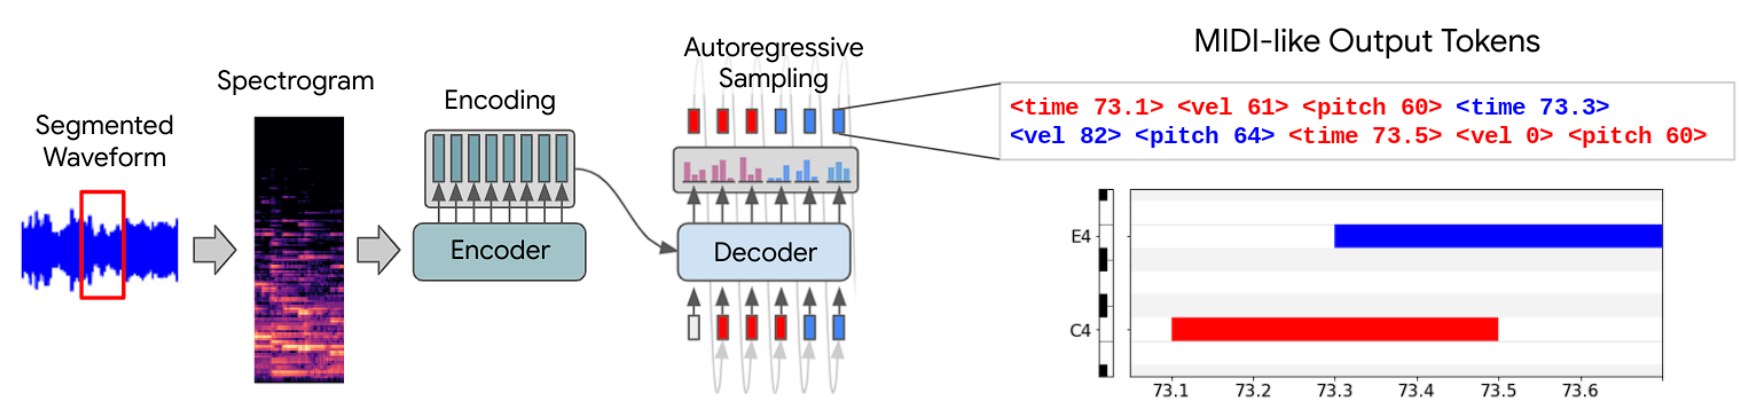
\includegraphics[width=1\textwidth]{Graphics/transcription_transformer}
    \caption[Verarbeitungspipeline des MT3-Modells]{Verarbeitungspipeline des Transformer-basierenden MT3-Modells  \cite{mt3colab}.}
    \label{fig:mt3_process}
\end{figure}

\subsection{Omnizart vs MT3}
Die beiden vorgestellten AMT-Systeme sind grundlegend verschieden aufgebaut.
Jetzt ist die Frage, welche dieser beiden Systeme ist besser geeignet
und unter welchen Voraussetzungen sollte man sich für welches System entscheiden.

Der größte Unterschied in der Architektur liegt darin,
das Omnizart verschiedenen KI-Modelle für unterschiedliche Aufgaben besitzt,
während MT3 ein einziges leistungsstarkes KI-Modell besitzt.
Somit kann man bei Omnizart leichter einen bestimmten Task verbessern oder analysieren.
Das ist vor allem gut, wenn man sich auf monophone Musikstücke konzentriert
und einen einfacheren Einstieg in die automatische Musiktranskription bekommen möchte.
Zudem gibt Omnizart eine größere Menge an Outputdaten zurück als MT3, bei dem nur eine MIDI-Datei ausgegeben wird.
MT3 hingegen besitzt ein einziges KI-Modell, wodurch man nicht gezielt einen speziellen Task umstrukturieren kann.
Dafür eignet sich das KI-Modell direkt wissen der verschiedenen Tasks an un kombiniert dieses.
Somit können polyphone Musikstücke deutliche besser transkribiert werden.
Durch YourMT3+ gibt es zudem weiteres Ausbaupotential, dahingegen entwickelt sich Omnizart nicht sonderlich weiter.

Bei den KI-Modellen hat MT3 einen klaren Vorsprung.
CNNs und GRUs sind schon seit längerem in AMT-Systemen vertreten.
Sie wurden ausgiebig angepasst und verbessert für diesen Anwendungsfall.
Hingegen zu diesen KI-Modellen ist das MT3 erst seit paar Jahren im Rennen.
Durch YourMT3+ wird es immer weiter entwickelt,
wodurch es in der nahen Zukunft zu einem Standard der automatischen Musiktranskription werden könnte.
Zudem ist das MT3-Modell deutlich besser auf polyphone Musikstücke ausgelegt.
In der mehrheit von Audiosignalen gibt es mehrere Stimmen.
Die meisten Menschen möchten auch lieber eine einfache Lösung, die wenig eigenaufwand benötigt.
Deshalb wäre ein zentrales KI-Modell, zur transkribierung von allen verschiedenen Audiosignalen, die populärste Lösung.
Ein Schwachpunkt des MT3-Modells ist der Rechenaufwand.
Da alles über ein KI-Modell läuft,
muss dieses umso mehr Rechenschritte durchführen und braucht exponentiell mehr GPU auslastung und Speicherkapazität.

Omnizart ist empfehlenswert, falls man sich gerade mit dem Forschungsgebiet neu auseinandersätz.
Man sieht viel schneller Fortschritte und kann sich erstmals auf kleiner KI-Modelle konzentrieren.
In den meisten anderen Fällen wäre jedoch das MT3-Modell, oder das Nachfolgermodell YourMT3+, empfohlen.
Dieses ist der State of the Art und wird auch noch in einigen Jahren Support erhalten.
Zudem ist man bei diesem Modell in keiner Weise eingeschränkt und kann jegliche Musik transkribieren.
Dieses Modell geht jedoch auch mit viel Rechenaufwand und einem guten Verständnis des Forschungsgebiets einher.
Deshalb sollte man sich, bevor man das MT3-Modell nutzt, gut damit auseinandergesetzt haben. % offen
\section{Fazit}
Automatische Musiktranskription entwickelt sich stetig weiter.
Besonders in den letzten Jahren hat dieses Forschungsgebiet erhebliche Fortschritte gemacht.
Verantwortlich dafür ist vor allem die rasante Entwicklung Künstlicher Intelligenz.
In nur wenigen Jahren wurden unzählige KI-Modelle entwickelt, die im Monatsrhythmus beachtliche Fortschritte zeigten.
Fast jedes Problem, was vorher durch Algorithmen gelöst wurde,
konnte durch ein schnelleres und besseres KI-Modell ersetzt werden.
Dies gilt auch für Algorithmen und Architekturen in AMT-Systemen.
CNNs und RNNs entwickelten sich in kürzester Zeit zum neuen Standard innerhalb der AMT-Forschung.

Dieses Phänomen ist jedoch erst der Anfang von Künstlicher Intelligenz und deren Anwendung in AMT-Systemen.
So schnell wie CNNs und RNNs die automatische Musiktranskription beeinflusst haben,
ebenso schnell treten bereits neue, verbesserte KI-Modelle auf den Plan.
Mit dem Transformer-basierten KI-Modell MT3 wurde erneut ein neuer Stand der Technik erreicht,
der die alten KI-Modelle ersetzten sollte.
Es ist zu erwarten, dass sich dieser Zyklus noch vielfach wiederholen wird,
da wir uns noch am Anfang der KI-Forschung befinden.

Trotz dieser großen Meilensteine gibt es in der automatischen Musiktranskription noch einige offene Probleme,
welche gelöst werden müssen.
Datensätze sind unzureichend, transkribierte Noten sind fehlerhaft oder unvollständig
und rauschende Audioaufnahmen verwirren die KI-Modelle zu stark.
KI-Modelle haben zahlreiche Probleme und Fehler beseitigt,
gleichzeitig öffneten sie neue Fehlerquellen, die zuvor nicht existierten.
Ein Beispiel dafür ist das sogenannte Blackbox-Verhalten moderner KI-Modelle.
Dadurch wird unklarer, was an dem Datensatz oder direkt in dem KI-Modell am besten verändert werden muss,
um ein besseres Ergebnis zu erzielen.

Eines der größten Herausforderungen bleibt jedoch die Überführung in lesbare Notenblätter.
Tatsächlich gibt es einige Tools und Firmen die diese Aufgabe mithilfe eines AMT-System versuchen zu lösen,
häufig sind die daraus resultierenden Notenblätter jedoch kaum brauchbar.
Die Noten werden nicht den richtigen Stimmen zugeordnet und Musikalische regeln werden nicht beachtet.
Das führt dazu, dass die Musiknoten nicht intuitiv spielbar sind.
Eine Lösung dafür wäre ein weiteres KI-Modell,
das sich mithilfe einer MIDI-Datei systematisch damit auseinandersetzt,
wie Musiknoten platziert werden müssen und wann Vorzeichen, Dynamikangaben sowie Artikulationszeichen gesetzt werden.

Im Ganzen ist die Einbindung von Künstlicher Intelligenz ein großer Fortschritt für die automatische Musiktranskription.
In naher Zukunft werden AMT-Systeme kontinuierlich weiterentwickelt
und in nicht allzu langer Zeit könnten diese auch im alltag eingesetzt werden.
 % Korrigiert

% --- Bibliography ---

\newpage
\printbibliography[heading=bibintoc, title={Literaturverzeichnis}]

% --- Document End ---

\end{document}
